

\section{名词解释}
\subsection{奥秘}

\subsubsection{天國的奧祕 太13:10-16/可4:10-12/路8:9-10}
\begin{itemize}
\item 門徒進前來，問耶穌說：「對眾人講話為什麼用比喻呢？」 11 耶穌回答說：「因為天國的奧祕只叫你們知道，不叫他們知道。 12 凡有的，還要加給他，叫他有餘；凡沒有的，連他所有的也要奪去。 13 所以我用比喻對他們講，是因他們看也看不見，聽也聽不見，也不明白。 14 在他們身上，正應了以賽亞的預言說：『你們聽是要聽見，卻不明白；看是要看見，卻不曉得。 15 因為這百姓油蒙了心，耳朵發沉，眼睛閉著，恐怕眼睛看見，耳朵聽見，心裡明白，回轉過來，我就醫治他們。』 16 但你們的眼睛是有福的，因為看見了；你們的耳朵也是有福的，因為聽見了。
\item 無人的時候，跟隨耶穌的人和十二個門徒問他這比喻的意思。 11 耶穌對他們說：「神國的奧祕只叫你們知道，若是對外人講，凡事就用比喻， 12 叫『他們看是看見，卻不曉得，聽是聽見，卻不明白；恐怕他們回轉過來，就得赦免』。」
\item 門徒問耶穌說：「這比喻是什麼意思呢？」 10 他說：「神國的奧祕只叫你們知道，至於別人，就用比喻，叫他們『看也看不見，聽也聽不明』。
\end{itemize}

\subsubsection{以色列人有幾分硬心的奧祕 羅11：25-32}
弟兄們，我不願意你們不知道這奧祕，恐怕你們自以為聰明，就是：以色列人有幾分是硬心的，等到外邦人的數目添滿了， 26 於是以色列全家都要得救。如經上所記：「必有一位救主從錫安出來，要消除雅各家的一切罪惡。」 27 又說：「我除去他們罪的時候，這就是我與他們所立的約。」 28 就著福音說，他們為你們的緣故是仇敵；就著揀選說，他們為列祖的緣故是蒙愛的。 29 因為神的恩賜和選召是沒有後悔的。 30 你們從前不順服神，如今因他們的不順服，你們倒蒙了憐恤。 31 這樣，他們也是不順服，叫他們因著施給你們的憐恤，現在也就蒙憐恤。 32 因為神將眾人都圈在不順服之中，特意要憐恤眾人。深哉，神豐富的智慧和知識！他的判斷何其難測，他的蹤跡何其難尋！ 34 「誰知道主的心，誰做過他的謀士呢？ 35 誰是先給了他，使他後來償還呢？」 36 因為萬有都是本於他，倚靠他，歸於他。願榮耀歸給他，直到永遠！阿們。
\subsubsection{福音和耶穌基督的奧祕 羅16：25-27}
唯有神能照我所傳的福音和所講的耶穌基督，並照永古隱藏不言的奧祕，堅固你們的心。 26 這奧祕如今顯明出來，而且按著永生神的命，藉眾先知的書指示萬國的民，使他們信服真道。 27 願榮耀因耶穌基督歸於獨一全智的神，直到永遠！阿們。

\subsubsection{各樣的奧祕 林前13:1-2/14:1-11}
\begin{itemize}
\item 我若能說萬人的方言，並天使的話語，卻沒有愛，我就成了鳴的鑼、響的鈸一般。 2 我若有先知講道之能，也明白\textcolor{red}{各樣的奧祕}、各樣的知識，而且有全備的信叫我能夠移山，卻沒有愛，我就算不得什麼。
\item 你們要追求愛，也要切慕屬靈的恩賜，其中更要羨慕的是做先知講道。 2 那說方言的原不是對人說，乃是對神說，因為沒有人聽出來，然而他在心靈裡卻是講說\textcolor{red}{各樣的奧祕}。 3 但做先知講道的是對人說，要造就、安慰、勸勉人。 4 說方言的是造就自己，做先知講道的乃是造就教會。 5 我願意你們都說方言，更願意你們做先知講道；因為說方言的若不翻出來，使教會被造就，那做先知講道的就比他強了。 6 弟兄們，我到你們那裡去，若只說方言，不用啟示或知識或預言或教訓給你們講解，我於你們有什麼益處呢？ 7 就是那有聲無氣的物，或簫或琴，若發出來的聲音沒有分別，怎能知道所吹所彈的是什麼呢？ 8 若吹無定的號聲，誰能預備打仗呢？ 9 你們也是如此，舌頭若不說容易明白的話，怎能知道所說的是什麼呢？這就是向空說話了。 10 世上的聲音或者甚多，卻沒有一樣是無意思的。 11 我若不明白那聲音的意思，這說話的人必以我為化外之人，我也以他為化外之人。
\end{itemize}

\subsubsection{奧祕的事 林前15:50-54}
弟兄們，我告訴你們說，血肉之體不能承受神的國，必朽壞的不能承受不朽壞的。 51 我如今把\textcolor{red}{一件奧祕的事}告訴你們：我們不是都要睡覺，乃是都要改變， 52 就在一霎時，眨眼之間，號筒末次吹響的時候。因號筒要響，死人要復活成為不朽壞的，我們也要改變。 53 這必朽壞的總要變成不朽壞的，這必死的總要變成不死的。 54 這必朽壞的既變成不朽壞的，這必死的既變成不死的，那時經上所記「死被得勝吞滅」的話就應驗了。

\subsubsection{神旨意的奧祕 弗1:3-14}
願頌讚歸於我們主耶穌基督的父神！他在基督裡曾賜給我們天上各樣屬靈的福氣， 4 就如神從創立世界以前在基督裡揀選了我們，使我們在他面前成為聖潔，無有瑕疵； 5 又因愛我們，就按著自己意旨所喜悅的，預定我們藉著耶穌基督得兒子的名分， 6 使他榮耀的恩典得著稱讚。這恩典是他在愛子裡所賜給我們的。 7 我們藉這愛子的血得蒙救贖，過犯得以赦免，乃是照他豐富的恩典。 8 這恩典是神用諸般智慧聰明，充充足足賞給我們的， 9 都是照他自己所預定的美意，叫我們知道他\textcolor{red}{旨意的奧祕}， 10 要照所安排的，在日期滿足的時候，使天上、地上一切所有的，都在基督裡面同歸於一。 11 我們也在他裡面得 a了基業，這原是那位隨己意行做萬事的，照著他旨意所預定的， 12 叫他的榮耀從我們這首先在基督裡有盼望的人，可以得著稱讚。 13 你們既聽見真理的道，就是那叫你們得救的福音，也信了基督，既然信他，就受了所應許的聖靈為印記。 14 這聖靈是我們得基業的憑據 b，直等到神之民 c被贖，使他的榮耀得著稱讚。

\subsubsection{福音的奧祕 弗3:1-9}
因此，我保羅——為你們外邦人做了基督耶穌被囚的，替你們祈禱。 2 諒必你們曾聽見神賜恩給我，將關切你們的職分託付我， 3 用啟示使我知道\textcolor{red}{福音的奧祕}，正如我以前略略寫過的。 4 你們念了，就能曉得我深知基督的奧祕。 5 這奧祕在以前的世代沒有叫人知道，像如今藉著聖靈啟示他的聖使徒和先知一樣。 6 這奧祕就是外邦人在基督耶穌裡，藉著福音，得以同為後嗣，同為一體，同蒙應許。 7 我做了這福音的執事，是照神的恩賜，這恩賜是照他運行的大能賜給我的。 8 我本來比眾聖徒中最小的還小，然而他還賜我這恩典，叫我把基督那測不透的豐富傳給外邦人， 9 又使眾人都明白，這歷代以來隱藏在創造萬物之神裡的奧祕是如何安排的， 10 為要藉著教會，使天上執政的、掌權的現在得知神百般的智慧。 11 這是照神從萬世以前在我們主基督耶穌裡所定的旨意。 12 我們因信耶穌，就在他裡面放膽無懼，篤信不疑地來到神面前。 13 所以，我求你們不要因我為你們所受的患難喪膽，這原是你們的榮耀。

\subsubsection{神的奧祕 林前2:1-16/啟10:5-7/11:15-19}
\begin{itemize}
\item 弟兄們，從前我到你們那裡去，並沒有用高言大智對你們宣傳神的奧祕。 2 因為我曾定了主意，在你們中間不知道別的，只知道耶穌基督並他釘十字架。 3 我在你們那裡，又軟弱，又懼怕，又甚戰兢。 4 我說的話、講的道，不是用智慧委婉的言語，乃是用聖靈和大能的明證， 5 叫你們的信不在乎人的智慧，只在乎神的大能。然而，在完全的人中，我們也講智慧，但不是這世上的智慧，也不是這世上有權有位將要敗亡之人的智慧。 7 我們講的，乃是從前所隱藏、神奧祕的智慧，就是神在萬世以前預定使我們得榮耀的。 8 這智慧，世上有權有位的人沒有一個知道的，他們若知道，就不把榮耀的主釘在十字架上了。 9 如經上所記：「神為愛他的人所預備的，是眼睛未曾看見，耳朵未曾聽見，人心也未曾想到的。」 10 只有神藉著聖靈向我們顯明了。因為聖靈參透萬事，就是神深奧的事也參透了。 11 除了在人裡頭的靈，誰知道人的事？像這樣，除了神的靈，也沒有人知道神的事。 12 我們所領受的，並不是世上的靈，乃是從神來的靈，叫我們能知道神開恩賜給我們的事。 13 並且我們講說這些事，不是用人智慧所指教的言語，乃是用聖靈所指教的言語，將屬靈的話解釋屬靈的事。然而，屬血氣的人不領會神聖靈的事，反倒以為愚拙；並且不能知道，因為這些事唯有屬靈的人才能看透。 15 屬靈的人能看透萬事，卻沒有一人能看透了他。 16 「誰曾知道主的心，去教導他呢？」但我們是有基督的心了。
\item 我所看見的那踏海踏地的天使向天舉起右手來， 6 指著那創造天和天上之物、地和地上之物、海和海中之物，直活到永永遠遠的，起誓說：「不再有時日了 a！ 7 但在第七位天使吹號發聲的時候，神的奧祕就成全了，正如神所傳給他僕人眾先知的佳音。」
\item 第七位天使吹號，天上就有大聲音說：「世上的國成了我主和主基督的國，他要做王，直到永永遠遠。」 16 在神面前、坐在自己位上的二十四位長老就面伏於地，敬拜神， 17 說：「昔在、今在的主神，全能者啊！我們感謝你，因你執掌大權做王了。 18 外邦發怒，你的憤怒也臨到了！審判死人的時候也到了！你的僕人眾先知和眾聖徒，凡敬畏你名的人，連大帶小得賞賜的時候也到了！你敗壞那些敗壞世界之人的時候也就到了！」當時，神天上的殿開了，在他殿中現出他的約櫃，隨後有閃電、聲音、雷轟、地震、大雹。
\end{itemize}

\subsubsection{神奧祕事的管家 林前4:1-5}
人應當以我們為基督的執事，為神奧祕事的管家。 2 所求於管家的，是要他有忠心。 3 我被你們論斷，或被別人論斷，我都以為極小的事，連我自己也不論斷自己。 4 我雖不覺得自己有錯，卻也不能因此得以稱義，但判斷我的乃是主。 5 所以，時候未到，什麼都不要論斷，只等主來，他要照出暗中的隱情，顯明人心的意念。那時，各人要從神那裡得著稱讚。

\subsubsection{七星和七個金燈臺的奧祕 啟示錄 1:20}
論到你所看見在我右手中的七星和七個金燈臺的奧祕，那七星就是七個教會的使者，七燈臺就是七個教會。
 
  which has been hidden

Ephesians 5:32 N-NNS
GRK: τὸ μυστήριον τοῦτο μέγα
NAS: This mystery is great;
KJV: is a great mystery: but I
INT: the mystery This great

Ephesians 6:19 N-ANS
GRK: γνωρίσαι τὸ μυστήριον τοῦ εὐαγγελίου
NAS: with boldness the mystery of the gospel,
KJV: to make known the mystery of the gospel,
INT: to make known the mystery of the gospel

Colossians 1:26 N-ANS
GRK: τὸ μυστήριον τὸ ἀποκεκρυμμένον
NAS: [that is], the mystery which has been hidden
KJV: [Even] the mystery which hath been hid
INT: the mystery which has been hidden

Colossians 1:27 N-GNS
GRK: δόξης τοῦ μυστηρίου τούτου ἐν
NAS: of this mystery among
KJV: of this mystery among
INT: glory of the mystery this among

Colossians 2:2 N-GNS
GRK: ἐπίγνωσιν τοῦ μυστηρίου τοῦ θεοῦ
NAS: of God's mystery, [that is], Christ
KJV: the acknowledgement of the mystery of God,
INT: [the] knowledge of the mystery of God

Colossians 4:3 N-ANS
GRK: λαλῆσαι τὸ μυστήριον τοῦ χριστοῦ
NAS: so that we may speak forth the mystery of Christ,
KJV: to speak the mystery of Christ,
INT: to speak the mystery of Christ

2 Thessalonians 2:7 N-NNS
GRK: τὸ γὰρ μυστήριον ἤδη ἐνεργεῖται
NAS: For the mystery of lawlessness
KJV: For the mystery of iniquity doth
INT: the indeed mystery already is working

1 Timothy 3:9 N-ANS
GRK: ἔχοντας τὸ μυστήριον τῆς πίστεως
NAS: [but] holding to the mystery of the faith
KJV: Holding the mystery of the faith in
INT: holding the mystery of the faith

1 Timothy 3:16 N-NNS
GRK: τῆς εὐσεβείας μυστήριον Ὃς ἐφανερώθη
NAS: great is the mystery of godliness:
KJV: great is the mystery of godliness: God
INT: of godliness mystery which was revealed

Revelation 1:20 N-NNS 

\subsection{奥秘}
\subsubsection{但以理書 2:22, 29-30, 46-48}
\begin{itemize} 
\itemsep-.25em
\item 2:22 他顯明\underline{深奧隱祕的事}，知道暗中所有的，光明也與他同居。
\item 2:29 王啊，你在床上想到後來的事，那顯明\underline{奧祕事}的主把將來必有的事指示你。至於那\underline{奧祕}的事顯明給我，並非因我的智慧勝過一切活人，乃為使王知道夢的講解和心裡的思念。
\item 46 當時尼布甲尼撒王俯伏在地，向但以理下拜，並且吩咐人給他奉上供物和香品。 47王對但以理說：「你既能顯明這\underline{奧祕}的事，你們的神誠然是萬神之神，萬王之主，又是顯明\underline{奧祕}事的。」 48於是王高抬但以理，賞賜他許多上等禮物，派他管理巴比倫全省，又立他為總理，掌管巴比倫的一切哲士
\end{itemize}

\subsubsection{阿摩司書 3:1-7}
1 「以色列人哪，你們全家是我從埃及地領上來的，當聽耶和華攻擊你們的話： 2 在地上萬族中我只認識你們，因此，我必追討你們的一切罪孽。 3 二人若不同心，豈能同行呢？ 4 獅子若非抓食，豈能在林中咆哮呢？少壯獅子若無所得，豈能從洞中發聲呢？ 5 若沒有機檻，雀鳥豈能陷在網羅裡呢？網羅若無所得，豈能從地上翻起呢？ 6 城中若吹角，百姓豈不驚恐呢？災禍若臨到一城，豈非耶和華所降的嗎？ 7 主耶和華若不將\underline{奧祕}指示他的僕人眾先知，就一無所行


\subsubsection{馬太福音 13:10-12, 13:35}
\begin{itemize} 
\itemsep-.25em
\item 10門徒進前來，問耶穌說：「對眾人講話為什麼用比喻呢？」 11耶穌回答說：「因為\underline{天國的奧祕}只叫你們知道，不叫他們知道。 12凡有的，還要加給他，叫他有餘；凡沒有的，連他所有的也要奪去。
\item 13:35 這是要應驗先知的話說：「我要開口用比喻，把創世以來所\underline{隱藏的事}發明出來。」
\end{itemize} 

\subsubsection{路加福音 8:10}
他說：「\underline{神國的奧祕}只叫你們知道，至於別人，就用比喻，叫他們『看也看不見，聽也聽不明』。

\subsubsection{羅馬書 2:16, 11:25, 16:25}
\begin{itemize} 
\itemsep-.25em
\item 就在神藉耶穌基督審判人\underline{隱祕事}的日子，照著我的福音所言。
\item 11:25 弟兄們，我不願意你們不知道這\underline{奧祕}，恐怕你們自以為聰明，就是：以色列人有幾分是硬心的，等到外邦人的數目添滿了，
\item 16:25 唯有神能照我所傳的福音和所講的耶穌基督，並照\underline{永古隱藏不言的奧祕}，堅固你們的心。
\end{itemize} 

\subsubsection{哥林多前書 2:1-13, 4:1-5, 14:1-3}
\begin{itemize} 
\itemsep-.25em
\item 1 弟兄們，從前我到你們那裡去，並沒有用高言大智對你們宣傳\underline{神的奧祕}。 2 因為我曾定了主意，在你們中間不知道別的，只知道耶穌基督並他釘十字架。 3 我在你們那裡，又軟弱，又懼怕，又甚戰兢。 4 我說的話、講的道，不是用智慧委婉的言語，乃是用聖靈和大能的明證， 5 叫你們的信不在乎人的智慧，只在乎神的大能。6 然而，在完全的人中，我們也講智慧，但不是這世上的智慧，也不是這世上有權有位將要敗亡之人的智慧。 7 我們講的，乃是\underline{從前所隱藏、神奧祕的智慧}，就是神在萬世以前預定使我們得榮耀的。 8 這智慧，世上有權有位的人沒有一個知道的，他們若知道，就不把榮耀的主釘在十字架上了。 9 如經上所記：「神為愛他的人所預備的，是眼睛未曾看見，耳朵未曾聽見，人心也未曾想到的。」 10 只有神藉著聖靈向我們顯明了。因為聖靈參透萬事，就是\underline{神深奧的事}也參透了。 11 除了在人裡頭的靈，誰知道人的事？像這樣，除了神的靈，也沒有人知道神的事。 12 我們所領受的，並不是世上的靈，乃是從神來的靈，叫我們能知道神開恩賜給我們的事。 13 並且我們講說這些事，不是用人智慧所指教的言語，乃是用聖靈所指教的言語，將屬靈的話解釋屬靈的事 。
\item 4:1 人應當以我們為基督的執事，為\underline{神奧祕事}的管家。 2 所求於管家的，是要他有忠心。 3 我被你們論斷，或被別人論斷，我都以為極小的事，連我自己也不論斷自己。 4 我雖不覺得自己有錯，卻也不能因此得以稱義，但判斷我的乃是主。 5 所以，時候未到，什麼都不要論斷，只等主來，他要照出暗中的隱情，顯明人心的意念。那時，各人要從神那裡得著稱讚。
\item 14:1 你們要追求愛，也要切慕屬靈的恩賜，其中更要羨慕的是做先知講道。 2那說方言的原不是對人說，乃是對神說，因為沒有人聽出來，然而他在心靈裡卻是講說各樣的\underline{奧祕}。 3但做先知講道的是對人說，要造就、安慰、勸勉人。
\end{itemize} 

\subsubsection{以弗所書 1:3-12, 3:3-4, 14:1-3}
\begin{itemize} 
\itemsep-.25em
\item 1:3 他在基督裡曾賜給我們天上各樣屬靈的福氣， 4 就如神從創立世界以前在基督裡揀選了我們，使我們在他面前成為聖潔，無有瑕疵； 5 又因愛我們，就按著自己意旨所喜悅的，預定我們藉著耶穌基督得兒子的名分， 6 使他榮耀的恩典得著稱讚。這恩典是他在愛子裡所賜給我們的。 7 我們藉這愛子的血得蒙救贖，過犯得以赦免，乃是照他豐富的恩典。 8 這恩典是神用諸般智慧聰明，充充足足賞給我們的， 9 都是照他自己所預定的美意，叫我們知道他\underline{旨意的奧祕}， 10 要照所安排的，在日期滿足的時候，使天上、地上一切所有的，都在基督裡面同歸於一。 11 我們也在他裡面得基業，這原是那位隨己意行做萬事的，照著他旨意所預定的， 12 叫他的榮耀從我們這首先在基督裡有盼望的人，可以得著稱讚。
\item 3:1 因此，我保羅——為你們外邦人做了基督耶穌被囚的，替你們祈禱 。 2 諒必你們曾聽見神賜恩給我，將關切你們的職分託付我， 3 用啟示使我知道\underline{福音的奧祕} ，正如我以前略略寫過的。你們念了，就能曉得我深知\underline{基督的奧祕} 。5 這\underline{奧祕}在以前的世代沒有叫人知道，像如今藉著聖靈啟示他的聖使徒和先知一樣。 6 這\underline{奧祕}就是外邦人在基督耶穌裡，藉著福音，得以同為後嗣，同為一體，同蒙應許。 7 我做了這福音的執事，是照神的恩賜，這恩賜是照他運行的大能賜給我的。 8我本來比眾聖徒中最小的還小，然而他還賜我這恩典，叫我把基督那測不透的豐富傳給外邦人， 9又使眾人都明白，這歷代以來隱藏在創造萬物之神\underline{裡的奧祕} 是如何安排的， 10為要藉著教會，使天上執政的、掌權的現在得知神百般的智慧。 11 這是照神從萬世以前在我們主基督耶穌裡所定的旨意。 12 我們因信耶穌，就在他裡面放膽無懼，篤信不疑地來到神面前。 13 所以，我求你們不要因我為你們所受的患難喪膽，這原是你們的榮耀。
\item  5:22 你們做妻子的，當順服自己的丈夫，如同順服主； 23 因為丈夫是妻子的頭，如同基督是教會的頭，他又是教會全體的救主。 24 教會怎樣順服基督，妻子也要怎樣凡事順服丈夫。 25 你們做丈夫的，要愛你們的妻子，正如基督愛教會，為教會捨己， 26 要用水藉著道把教會洗淨，成為聖潔， 27 可以獻給自己，做個榮耀的教會，毫無玷汙、皺紋等類的病，乃是聖潔沒有瑕疵的。 28 丈夫也當照樣愛妻子，如同愛自己的身子，愛妻子便是愛自己了。 29 從來沒有人恨惡自己的身子，總是保養顧惜，正像基督待教會一樣， 30 因我們是他身上的肢體 。 31 為這個緣故，人要離開父母，與妻子聯合，二人成為一體。 32這是\underline{極大的奧祕} ，但我是指著基督和教會說的。 33然而你們各人都當愛妻子，如同愛自己一樣；妻子也當敬重她的丈夫。
\item 6:18靠著聖靈，隨時多方禱告祈求，並要在此警醒不倦，為眾聖徒祈求； 19也為我祈求，使我得著口才，能以放膽開口講明\underline{福音的奧祕}—— 20我為這\underline{福音的奧祕} 做了戴鎖鏈的使者——並使我照著當盡的本分放膽講論。
\end{itemize} 

\subsubsection{歌羅西書 1:25-27}
25我照神為你們所賜我的職分做了教會的執事，要把神的道理傳得全備。 26這道理就是歷世歷代所隱藏的奧祕，但如今向他的聖徒顯明了。 27神願意叫他們知道，這奧祕在外邦人中有何等豐盛的榮耀，就是基督在你們心裡成了有榮耀的盼望。
歌羅西書 2:2
要叫他們的心得安慰，因愛心互相聯絡，以致豐豐足足在悟性中有充足的信心，使他們真知神的奧祕，就是基督，
歌羅西書 3:3
因為你們已經死了，你們的生命與基督一同藏在神裡面。
歌羅西書 4:3
也要為我們禱告，求神給我們開傳道的門，能以講基督的奧祕——我為此被捆鎖——

提摩太前書 3:9
8做執事的也是如此，必須端莊，不一口兩舌，不好喝酒，不貪不義之財； 9要存清潔的良心，固守真道的奧祕。 10這等人也要先受試驗，若沒有可責之處，然後叫他們做執事

啟示錄 10:7
但在第七位天使吹號發聲的時候，神的奧祕就成全了，正如神所傳給他僕人眾先知的佳音。」
啟示錄 11:15
第七位天使吹號，天上就有大聲音說：「世上的國成了我主和主基督的國，他要做王，直到永永遠遠。」

啟示錄 17:7
7天使對我說：「你為什麼稀奇呢？我要將這女人和馱著她的那七頭十角獸的奧祕告訴你。 8你所看見的獸，先前有，如今沒有，將要從無底坑裡上來，又要歸於沉淪。凡住在地上，名字從創世以來沒有記在生命冊上的，見先前有、如今沒有、以後再有的獸，就必稀奇












\subsection{巴比倫}

\subsubsection{耶利米書 51：54-58}
54 有哀號的聲音從\underline{巴比倫}出來，有大毀滅的響聲從迦勒底人之地發出。 55 因耶和華使\underline{巴比倫}變為荒場，使其中的大聲滅絕。仇敵彷彿眾水，波浪砰訇，響聲已經發出。 56 這是行毀滅的臨到\underline{巴比倫}，巴比倫的勇士被捉住，他們的弓折斷了，因為耶和華是施行報應的神，必定施行報應。 57 君王，名為萬軍之耶和華的說：「我必使\underline{巴比倫}的首領、智慧人、省長、副省長和勇士都沉醉，使他們睡了長覺永不醒起。」 58 萬軍之耶和華如此說：「\underline{巴比倫}寬闊的城牆必全然傾倒，她高大的城門必被火焚燒。眾民所勞碌的必致虛空，列國所勞碌的被火焚燒，他們都必困乏。」





\subsection{白马}
\subsubsection{白马(啟 3:10, 6:1-2, 19:11-21/撒迦利亞書 1:7-11, 6:1-8)}
\begin{itemize}
\itemsep-.25em
\item 啟示錄
\begin{itemize}
\itemsep-.25em
\item 3:10 『你既遵守我忍耐的道，我必在普天下人受試煉的時候，保守你免去你的試煉。 11 我必快來！你要持守你所有的，免得人奪去你的\underline{冠冕}。
\item 6:1-2: 我看見羔羊揭開七印中第一印的時候，就聽見四活物中的一個活物聲音如雷說：「你來！」 2 我就觀看，見有一匹\underline{白馬}。騎在馬上的拿著弓，並有\underline{冠冕}賜給他，他便出來，勝了又要勝。
\item 19:11-21: 我觀看，見天開了。有一匹白馬，騎在馬上的稱為「誠信真實」，他審判、爭戰都按著公義。 12 他的眼睛如火焰，他頭上戴著許多冠冕，又有寫著的名字，除了他自己沒有人知道。 13 他穿著濺了血的衣服，他的名稱為「神之道」。 14 在天上的眾軍騎著白馬，穿著細麻衣，又白又潔，跟隨他。 15 有利劍從他口中出來，可以擊殺列國。他必用鐵杖轄管 b他們，並要踹全能神烈怒的酒榨。 16 在他衣服和大腿上有名寫著說：「萬王之王，萬主之主。」17 我又看見一位天使站在日頭中，向天空所飛的鳥大聲喊著說：「你們聚集來赴神的大筵席！ 18 可以吃君王與將軍的肉，壯士與馬和騎馬者的肉，並一切自主的、為奴的，以及大小人民的肉。」19 我看見那獸和地上的君王，並他們的眾軍都聚集，要與騎白馬的並他的軍兵爭戰。 20 那獸被擒拿，那在獸面前曾行奇事、迷惑受獸印記和拜獸像之人的假先知，也與獸同被擒拿。他們兩個就活活地被扔在燒著硫磺的火湖裡。 21 其餘的被騎白馬者口中出來的劍殺了。飛鳥都吃飽了他們的肉。
\end{itemize}
\item 撒迦利亞書
\begin{itemize}
\itemsep-.25em
\item 1:7-11 大流士第二年十一月，就是細罷特月二十四日，耶和華的話臨到易多的孫子、比利家的兒子先知撒迦利亞說： 8 我夜間觀看，見一人騎著紅馬，站在窪地番石榴樹中間，在他身後又有\underline{紅馬、黃馬和白馬}。 9 我對與我說話的天使說：「主啊，這是什麼意思？」他說：「我要指示你這是什麼意思。」 10 那站在番石榴樹中間的人說：\underline{「這是奉耶和華差遣在遍地走來走去的。」} 11 那些騎馬的對站在番石榴樹中間耶和華的使者說：「我們已在遍地走來走去，見全地都安息平靜。」
\item 6:1-8 我又舉目觀看，見有四輛車從兩山中間出來，那山是銅山。 2 第一輛車套著紅馬，第二輛車套著黑馬， 3 第三輛車套著白馬，第四輛車套著有斑點的壯馬。 4 我就問與我說話的天使說：「主啊，這是什麼意思？」 5 天使回答我說：「這是天的四風，是從普天下的主面前出來的。 6 套著黑馬的車往北方去，白馬跟隨在後，有斑點的馬往南方去。」 7 壯馬出來，要在遍地走來走去。天使說：「你們只管在遍地走來走去。」牠們就照樣行了。 8 他又呼叫我說：「看哪，\underline{往北方去的(黑馬白馬)已在北方安慰我的心。}」
\end{itemize}
\end{itemize}

\subsubsection{拿著弓(詩篇 78:9, 王下 13:17, 耶 50:14, 51:3,創49:22-24)}
\begin{itemize}
\itemsep-.25em
\item 詩篇 78:9: 以法蓮的子孫帶著兵器拿著弓，不要像他們的祖宗，是頑梗悖逆居心不正之輩，向著神心不誠實。以法蓮的子孫帶著兵器拿著弓，臨陣之日轉身退後。他們不遵守神的約，不肯
\item 列王紀下 13:17 說：「你開朝東的窗戶。」他就開了。以利沙說：「射箭吧。」他就射箭。以利沙說：「這是耶和華的得勝箭，就是戰勝亞蘭人的箭。因為你必在亞弗攻打亞蘭人，直到滅盡他們。」
\item 耶利米书
\begin{itemize}
\itemsep-.25em
\item 50:14 所有拉弓的，你們要在巴比倫的四圍擺陣，射箭攻擊她，不要愛惜箭枝，因她得罪了耶和華。
\item 51:3 我要打發外邦人來到巴比倫，簸揚她，使她的地空虛，在她遭禍的日子他們要周圍攻擊她。拉弓的要向拉弓的和貫甲挺身的射箭，不要憐惜她的少年人，要滅盡她的全軍。
\end{itemize}
\item 創 49:22-24: 22約瑟是多結果子的樹枝，是泉旁多結果的枝子，他的枝條探出牆外。弓箭手將他苦害，向他射箭，逼迫他。24 但他的弓仍舊堅硬，他的手健壯敏捷，這是因以色列的牧者，以色列的磐石，就是雅各的大能者。
\end{itemize}

\subsubsection{箭(賽 49:1-13, 撒迦利亞書 9:14 ,哈巴谷書 9:2-15)}
\begin{description}
\item 以賽亞書 49:1-13 \\
「眾海島啊，當聽我言！遠方的眾民哪，留心而聽！自我出胎，耶和華就選召我；自出母腹，他就提我的名。 2 他使我的口如快刀，將我藏在他手蔭之下；又使我成為磨亮的箭，將我藏在他箭袋之中。 3 對我說：『你是我的僕人以色列，我必因你得榮耀。』 4 我卻說：『我勞碌是徒然，我盡力是虛無虛空，然而我當得的理必在耶和華那裡，我的賞賜必在我神那裡。』5 「耶和華從我出胎造就我做他的僕人，要使雅各歸向他，使以色列到他那裡聚集。原來耶和華看我為尊貴，我的神也成為我的力量。 6 現在他說：『你做我的僕人，使雅各眾支派復興，使以色列中得保全的歸回，尚為小事，我還要使你做外邦人的光，叫你施行我的救恩，直到地極。』」 7 救贖主以色列的聖者耶和華，對那被人所藐視、本國所憎惡、官長所虐待的如此說：「君王要看見就站起，首領也要下拜，都因信實的耶和華，就是揀選你以色列的聖者。」8 耶和華如此說：「在悅納的時候，我應允了你；在拯救的日子，我濟助了你。我要保護你，使你做眾民的中保 a，復興遍地，使人承受荒涼之地為業。 9 對那被捆綁的人說：『出來吧！』對那在黑暗的人說：『顯露吧！』他們在路上必得飲食，在一切淨光的高處必有食物。 10 不飢不渴，炎熱和烈日必不傷害他們，因為憐恤他們的必引導他們，領他們到水泉旁邊。 11 我必使我的眾山成為大道，我的大路也被修高。 12 看哪，這些從遠方來，這些從北方，從西方來，這些從秦 b國來。」 13 諸天哪，應當歡呼！大地啊，應當快樂！眾山哪，應當發聲歌唱！因為耶和華已經安慰他的百姓，也要憐恤他困苦之民。
\item 撒迦利亞書 9:14 \\耶和華必顯現在他們以上，他的箭必射出像閃電。主耶和華必吹角，乘南方的旋風而行。
\item 哈巴谷書 9:2-15 \\耶和華啊，我聽見你的名聲就懼怕。耶和華啊，求你在這些年間復興你的作為，在這些年間顯明出來，在發怒的時候以憐憫為念。 3 神從提幔而來，聖者從巴蘭山臨到。（細拉）他的榮光遮蔽諸天，頌讚充滿大地。 4 他的輝煌如同日光，從他手裡射出光線，在其中藏著他的能力。 5 在他前面有瘟疫流行，在他腳下有熱症發出。 6 他站立，量了大地；觀看，趕散萬民。永久的山崩裂，長存的嶺塌陷，他的作為與古時一樣。 7 我見古珊的帳篷遭難，米甸的幔子戰兢。 8 耶和華啊，你乘在馬上，坐在得勝的車上，豈是不喜悅江河，向江河發怒氣，向洋海發憤恨嗎？ 9 你的弓全然顯露，向眾支派所起的誓都是可信的。（細拉）你以江河分開大地。 10 山嶺見你，無不戰懼；大水氾濫過去，深淵發聲，洶湧翻騰 c。 11 因你的箭射出發光，你的槍閃出光耀，日月都在本宮停住。 12 你發憤恨通行大地，發怒氣責打列國如同打糧。 13 你出來要拯救你的百姓，拯救你的受膏者，打破惡人家長的頭，露出他的腳 d，直到頸項。（細拉） 14 你用敵人的戈矛刺透他戰士的頭，他們來如旋風，要將我們分散，他們所喜愛的是暗中吞吃貧民。 15 你乘馬踐踏紅海，就是踐踏洶湧的大水。
\end{description}
\subsubsection{冠冕(林前9:25/啟 3:11/希 2:7/提後2:4/彼前5:4)}
\begin{itemize}
\itemsep-.25em
\item 哥林多前書 9:25 凡較力爭勝的，諸事都有節制。他們不過是要得能壞的冠冕，我們卻是要得不能壞的冠冕。
\item 提摩太後書 2:4 凡在軍中當兵的，不將世務纏身，好叫那招他當兵的人喜悅人若在場上比武，非按規矩，就不能得冠冕。
\item 啟示錄 3:11 我必快來！你要持守你所有的，免得人奪去你的冠冕。
\item 希伯來書 2:7 你叫他比天使微小一點，賜他榮耀、尊貴為冠冕，並將你手所造的都派他管理，
\item 彼得前書 5:4 到了牧長顯現的時候，你們必得那永不衰殘的榮耀冠冕。
\end{itemize}
\subsubsection{勝了又要勝 (啟13:1-6)}
我又看見一個獸從海中上來，有十角七頭，在十角上戴著十個冠冕，七頭上有褻瀆的名號。 2 我所看見的獸形狀像豹，腳像熊的腳，口像獅子的口。那龍將自己的能力、座位和大權柄都給了牠。 3 我看見獸的七頭中，有一個似乎受了死傷，那死傷卻醫好了。全地的人都稀奇，跟從那獸， 4 又拜那龍，因為牠將自己的權柄給了獸，也拜獸，說：「誰能比這獸，誰能與牠交戰呢？」 5 又賜給牠說誇大褻瀆話的口，又有權柄賜給牠，可以任意而行四十二個月。 6 獸就開口向神說褻瀆的話，褻瀆神的名並他的帳幕，以及那些住在天上的。又任憑牠與聖徒爭戰，並且得勝；也把權柄賜給牠，制伏各族、各民、各方、各國。






\subsection{白石(一塊)——別迦摩}

\subsubsection{神改的名字-亞伯拉罕,撒拉,雅各}
\begin{itemize} 
\itemsep-.25em
\item 創世記 17：1-8
亞伯蘭年九十九歲的時候，耶和華向他顯現，對他說：「我是全能的神，你當在我面前做完全人。 2 我就與你立約，使你的後裔極其繁多。」 3 亞伯蘭俯伏在地，神又對他說： 4 「我與你立約：你要做多國的父。 5 從此以後，你的名不再叫亞伯蘭，要叫亞伯拉罕，因為我已立你做多國的父。 6 我必使你的後裔極其繁多，國度從你而立，君王從你而出。 7 我要與你並你世世代代的後裔堅立我的約，做永遠的約，是要做你和你後裔的神。 8 我要將你現在寄居的地，就是迦南全地，賜給你和你的後裔永遠為業，我也必做他們的神。」
\item 創世記 17：15-16，19
神又對亞伯拉罕說：「你的妻子撒萊，不可再叫撒萊，她的名要叫撒拉。 16 我必賜福給她，也要使你從她得一個兒子。我要賜福給她，她也要做多國之母，必有百姓的君王從她而出。」 19神說：「不然，你妻子撒拉要給你生一個兒子，你要給他起名叫以撒。我要與他堅定所立的約，做他後裔永遠的約。
\item 創世記 32:27-29
…27那人說：「你名叫什麼？」他說：「我名叫雅各。」 28那人說：「你的名不要再叫雅各，要叫以色列，因為你與神與人較力，都得了勝。」 29雅各問他說：「請將你的名告訴我。」那人說：「何必問我的名？」於是在那裡給雅各祝福。
\item 創世記 35:9-11
雅各從巴旦亞蘭回來，神又向他顯現，賜福於他， 10且對他說：「你的名原是雅各，從今以後不要再叫雅各，要叫以色列。」這樣，他就改名叫以色列。 11神又對他說：「我是全能的神。你要生養眾多，將來有一族和多國的民從你而生，又有君王從你而出。
\item 列王紀上 18:31
以利亞照雅各子孫支派的數目，取了十二塊石頭（耶和華的話曾臨到雅各說「你的名要叫以色列」），
\end{itemize} 

\subsubsection{神赐的名字-亞當,何西阿的三个孩子，耶底底亞，以賽亞儿子}
\begin{itemize} 
\itemsep-.25em
\item 亞當的名字是神给取的。
\item 撒母耳記下 12：24-25
大衛安慰他的妻拔示巴，與她同寢，她就生了兒子，給他起名叫所羅門。耶和華也喜愛他，25就藉先知拿單賜他一個名字，叫耶底底亞，因為耶和華愛他
\item 以賽亞書 8:1-4
耶和華對我說：「你取一塊大板子，拿人的筆，寫上『瑪黑珥‧沙拉勒‧哈施‧罷斯』。 2 我要用可靠的證人，烏利亞祭司和耶比利家的兒子撒迦利亞為我作證。」「瑪黑珥‧沙拉勒‧哈施‧罷斯」意思是「擄掠速臨、搶奪即將發生」。3 我親近女先知；她就懷孕生子，耶和華對我說：「給他起名叫瑪黑珥‧沙拉勒‧哈施‧罷斯； 4 因為在這孩子還不曉得叫爸爸媽媽以前，大馬士革的財寶和撒瑪利亞的擄物必被亞述王掠奪一空。」
\item 何西阿书 1：4-9
耶和华就对何西阿说：“给他起名叫耶斯列；因为不久我就要惩罚耶户家在耶斯列流人血的罪，我要灭绝以色列家的国。5 “到那日，我要在耶斯列平原折断以色列的弓。”6 后来，歌玛又怀孕，生了一个女儿。耶和华对何西阿说：“给她起名叫罗．路哈玛（“罗．路哈玛”意即“不蒙怜恤”）；因为我必不再怜恤以色列家，我决不赦免他们。7 “但我要怜恤犹大家，使他们靠耶和华他们的　神得救。我要拯救他们，并不是靠弓、靠刀、靠战争，也不是靠战马、靠骑兵。”8 罗．路哈玛断奶之后，歌玛又怀孕生了一个儿子。9 耶和华说：“给他起名叫罗．阿米（“罗．阿米”意即“非我民”）；因为你们不是我的子民，我也不是你们的神。
\end{itemize}

\subsubsection{新约中神赐的名字人-耶穌,磯法,约翰}
\begin{itemize} 
\itemsep-.25em
\item 馬太福音 1：18-25
18 耶穌基督降生的事記在下面：他母親馬利亞已經許配了約瑟，還沒有迎娶，馬利亞就從聖靈懷了孕。 19 她丈夫約瑟是個義人，不願意明明地羞辱她，想要暗暗地把她休了。 20 正思念這事的時候，有主的使者向他夢中顯現，說：「大衛的子孫約瑟，不要怕，只管娶過你的妻子馬利亞來，因她所懷的孕是從聖靈來的。 21 她將要生一個兒子，你要給他起名叫耶穌，因他要將自己的百姓從罪惡裡救出來。」 22 這一切的事成就，是要應驗主藉先知所說的話說： 23 「必有童女懷孕生子，人要稱他的名為以馬內利。」（「以馬內利」翻出來就是「神與我們同在」。） 24 約瑟醒了，起來，就遵著主使者的吩咐把妻子娶過來， 25 只是沒有和她同房，等她生了兒子，就給他起名叫耶穌。
\item 約翰福音 1： 42 於是領他去見耶穌。耶穌看著他說：「你是約翰的兒子西門，你要稱為磯法。」（「磯法」翻出來就是「彼得」。）
\item 路加福音 1:8-23 8 撒迦利亞按班次在神面前供祭司的職分， 9 照祭司的規矩掣籤，得進主殿燒香。 10 燒香的時候，眾百姓在外面禱告。 11 有主的使者站在香壇的右邊向他顯現。 12 撒迦利亞看見，就驚慌害怕。 13 天使對他說：「撒迦利亞，不要害怕，因為你的祈禱已經被聽見了。你的妻子伊利莎白要給你生一個兒子，你要給他起名叫約翰。 14 你必歡喜快樂，有許多人因他出世也必喜樂。 15 他在主面前將要為大，淡酒濃酒都不喝，從母腹裡就被聖靈充滿了。 16 他要使許多以色列人回轉，歸於主他們的神。 17 他必有以利亞的心志能力，行在主的前面，叫為父的心轉向兒女，叫悖逆的人轉從義人的智慧，又為主預備合用的百姓。」 18 撒迦利亞對天使說：「我憑著什麼可知道這事呢？我已經老了，我的妻子也年紀老邁了。」 19 天使回答說：「我是站在神面前的加百列，奉差而來對你說話，將這好信息報給你。 20 到了時候，這話必然應驗。只因你不信，你必啞巴，不能說話，直到這事成就的日子。」 21 百姓等候撒迦利亞，詫異他許久在殿裡。 22 及至他出來，不能和他們說話，他們就知道他在殿裡見了異象，因為他直向他們打手勢，竟成了啞巴。 23 他供職的日子已滿，就回家去了。
\end{itemize} 

\subsubsection{名字}
\begin{itemize} 
\itemsep-.25em
\item 以賽亞書 1:26
我也必復還你的審判官，像起初一樣；復還你的謀士，像起先一般。然後你必稱為公義之城，忠信之邑。」
\item 以賽亞書 43:1-7
1 雅各啊，創造你的耶和華，以色列啊，造成你的那位，現在如此說：「你不要害怕，因為我救贖了你；我曾提你的名召你，你是屬我的。 2 你從水中經過，我必與你同在；你趟過江河，水必不漫過你；你從火中行過，必不被燒，火焰也不著在你身上。 3 因為我是耶和華你的神，是以色列的聖者，你的救主。我已經使埃及做你的贖價，使古實和西巴代替你。 4 因我看你為寶為尊，又因我愛你，所以我使人代替你，使列邦人替換你的生命。 5 不要害怕，因我與你同在。我必領你的後裔從東方來，又從西方招聚你。 6 我要對北方說『交出來！』，對南方說『不要拘留！』，將我的眾子從遠方帶來，將我的眾女從地極領回， 7 就是凡稱為我名下的人，是我為自己的榮耀創造的，是我所做成、所造做的。」
\item 以賽亞書 48:19
你的後裔也必多如海沙，你腹中所生的也必多如沙粒，他的名在我面前必不剪除，也不滅絕。」
\item 以賽亞書 55:13
松樹長出代替荊棘，番石榴長出代替蒺藜，這要為耶和華留名，作為永遠的證據，不能剪除。」
\item 以賽亞書 56：1-5
1 耶和華如此說：「你們當守公平，行公義，因我的救恩臨近，我的公義將要顯現。 2 謹守安息日而不干犯，禁止己手而不作惡，如此行、如此持守的人，便為有福！」 3 與耶和華聯合的外邦人不要說：「耶和華必定將我從他民中分別出來。」太監也不要說：「我是枯樹。」 4 因為耶和華如此說：「那些謹守我的安息日，揀選我所喜悅的事，持守我約的太監， 5 我必使他們在我殿中、在我牆內有紀念，有名號，比有兒女的更美。我必賜他們永遠的名，不能剪除。
\item 以賽亞書 60:18
你地上不再聽見強暴的事，境內不再聽見荒涼毀滅的事。你必稱你的牆為『拯救』，稱你的門為『讚美』。
\item 以賽亞書 62：1-5
1我因錫安必不靜默，為耶路撒冷必不息聲，直到他的公義如光輝發出，他的救恩如明燈發亮。 2列國必見你的公義，列王必見你的榮耀。你必得新名的稱呼，是耶和華親口所起的。 你在耶和華的手中要作為華冠，在你神的掌上必作為冕旒。 4 你必不再稱為「撇棄的」，你的地也不再稱為「荒涼的」，你卻要稱為「我所喜悅的」，你的地也必稱為「有夫之婦」，因為耶和華喜悅你，你的地也必歸他。 5 少年人怎樣娶處女，你的眾民 a也要照樣娶你；新郎怎樣喜悅新婦，你的神也要照樣喜悅你。
\item 以賽亞書 66:22
耶和華說：「我所要造的新天新地怎樣在我面前長存，你們的後裔和你們的名字也必照樣長存。
\item 西番雅書 3:20
那時，我必領你們進來，聚集你們。我使你們被擄之人歸回的時候，就必使你們在地上的萬民中有名聲，得稱讚。」這是耶和華說的。
\item 以弗所書 3：14-19
因此，我在父面前屈膝—— 15 天上地上的各家，都是從他得名—— 16 求他按著他豐盛的榮耀，藉著他的靈，叫你們心裡的力量剛強起來， 17 使基督因你們的信住在你們心裡，叫你們的愛心有根有基， 18 能以和眾聖徒一同明白基督的愛是何等長闊高深， 19 並知道這愛是過於人所能測度的，便叫神一切所充滿的充滿了你們。
\item 啟示錄 2:17
聖靈向眾教會所說的話，凡有耳的，就應當聽！得勝的，我必將那隱藏的嗎哪賜給他，並賜他一塊白石，石上寫著新名，除了那領受的以外，沒有人能認識。』
\item 啟示錄 3:12
得勝的，我要叫他在我神殿中做柱子，他也必不再從那裡出去。我又要將我神的名和我神城的名——這城就是從天上、從我神那裡降下來的新耶路撒冷——並我的新名，都寫在他上面。
\item 啟示錄 19:12
他的眼睛如火焰，他頭上戴著許多冠冕，又有寫著的名字，除了他自己沒有人知道。
\item 啟示錄 19:16
有利劍從他口中出來，可以擊殺列國。他必用鐵杖轄管他們，並要踹全能神烈怒的酒榨。 16在他衣服和大腿上有名寫著說：「萬王之王，萬主之主。」
\end{itemize} 





\subsection{被提726 $\grave{\alpha}$$\rho$$\pi
$$\acute{\alpha}$$\zeta$$\omega$}

\subsubsection{馬太福音 11：11-19 $\grave{\alpha}$$\rho$$\pi$$\acute{\alpha}$$\zeta$$o$$\upsilon$$\sigma$$\iota$$\nu$}
「我實在告訴你們：凡婦人所生的，沒有一個興起來大過施洗約翰的；然而天國裡最小的比他還大。 12 從施洗約翰的時候到如今，天國是努力進入的，努力的人就\underline{得著$\grave{\alpha}$$\rho$$\pi$$\acute{\alpha}$$\zeta$$o$$\upsilon$$\sigma$$\iota$$\nu$}了。 13 因為眾先知和律法說預言到約翰為止； 14 你們若肯領受，這人就是那應當來的以利亞。 15 有耳可聽的，就應當聽！ 16 我可用什麼比這世代呢？好像孩童坐在街市上招呼同伴說： 17 『我們向你們吹笛，你們不跳舞！我們向你們舉哀，你們不捶胸！』 18 約翰來了，也不吃也不喝，人就說他是被鬼附著的。 19 人子來了，也吃也喝，人又說他是貪食好酒的人，是稅吏和罪人的朋友。但智慧之子總以智慧為是。」

\subsubsection{馬太福音 12：25-30 $\grave{\alpha}$$\rho$$\pi$$\acute{\alpha}$$\sigma$$\alpha$$\iota$}
25 耶穌知道他們的意念，就對他們說：「凡一國自相紛爭，就成為荒場；一城一家自相紛爭，必站立不住。 26 若撒旦趕逐撒旦，就是自相紛爭，他的國怎能站得住呢？ 27 我若靠著別西卜趕鬼，你們的子弟趕鬼又靠著誰呢？這樣，他們就要斷定你們的是非。 28 我若靠著神的靈趕鬼，這就是神的國臨到你們了。 29 人怎能進壯士家裡\underline{搶奪$\grave{\alpha}$$\rho$$\pi$$\acute{\alpha}$$\sigma$$\alpha$$\iota$ἁρπάσαι}他的家具呢？除非先捆住那壯士，才可以搶奪他的家財。 30 不與我相合的，就是敵我的；不同我收聚的，就是分散的。

\subsubsection{使徒行傳 8：36-40 $\acute{\eta}$$\rho$$\pi$$\alpha$$\sigma$$\epsilon$$\nu$}
36 二人正往前走，到了有水的地方，太監說：「看哪，這裡有水！我受洗有什麼妨礙呢？」 38 於是吩咐車站住，腓利和太監二人同下水裡去，腓利就給他施洗。 39 從水裡上來，主的靈把腓利\underline{提 $\acute{\eta}$$\rho$$\pi$$\alpha$$\sigma$$\epsilon$$\nu$ ἥρπασεν}了去。太監也不再見他了，就歡歡喜喜地走路。 40 後來有人在亞鎖都遇見腓利；他走遍那地方，在各城宣傳福音，直到愷撒利亞。

\subsubsection{哥林多後書 12：1-4 $\grave{\alpha}$$\rho$$\pi$$\alpha$$\gamma$$\acute{\epsilon}$$\nu$$\tau$$\alpha$, $\grave{\eta}$$\rho$$\pi$$\acute{\alpha}$$\gamma$$\eta$}
1 我自誇固然無益，但我是不得已的。如今我要說到主的顯現和啟示。 2 我認得一個在基督裡的人，他前十四年被\underline{提$\grave{\alpha}$$\rho$$\pi$$\alpha$$\gamma$$\acute{\epsilon}$$\nu$$\tau$$\alpha$ἁρπαγέντα}到第三層天上去——或在身內，我不知道；或在身外，我也不知道；只有神知道。 3 我認得這人——或在身內、或在身外，我都不知道，只有神知道—— 4 他被\underline{提$\grave{\eta}$$\rho$$\pi$$\acute{\alpha}$$\gamma$$\eta$ἡρπάγη}到樂園裡，聽見隱祕的言語，是人不可說的。

\subsubsection{帖撒羅尼迦前書 4：13-18 $\grave{\alpha}$$\rho$$\pi$$\alpha$$\gamma$$\eta$$\sigma$$\acute{o}$$\mu$$\epsilon$$\theta$$\alpha$}
論到睡了的人，我們不願意弟兄們不知道，恐怕你們憂傷，像那些沒有指望的人一樣。 14 我們若信耶穌死而復活了，那已經在耶穌裡睡了的人，神也必將他們與耶穌一同帶來。 15 我們現在照主的話告訴你們一件事：我們這活著還存留到主降臨的人，斷不能在那已經睡了的人之先。 16 因為主必親自從天降臨，有呼叫的聲音和天使長的聲音，又有神的號吹響，那在基督裡死了的人必先復活， 17 以後我們這活著還存留的人必和他們一同被\underline{提 $\grave{\alpha}$$\rho$$\pi$$\alpha$$\gamma$$\eta$$\sigma$$\acute{o}$$\mu$$\epsilon$$\theta$$\alpha$ἁρπαγησόμεθα}到雲裡，在空中與主相遇；這樣，我們就要和主永遠同在。 18 所以，你們當用這些話彼此勸慰。

\subsubsection{啟示錄 12：3-6 $\grave{\eta}$$\rho$$\pi$$\acute{\alpha}$$\sigma$$\theta$$\eta$}
3 天上又現出異象來：有一條大紅龍，七頭十角，七頭上戴著七個冠冕， 4 牠的尾巴拖拉著天上星辰的三分之一，摔在地上。龍就站在那將要生產的婦人面前，等她生產之後，要吞吃她的孩子。 5 婦人生了一個男孩子，是將來要用鐵杖轄管萬國的；她的孩子被\underline{提 $\grave{\eta}$$\rho$$\pi$$\acute{\alpha}$$\sigma$$\theta$$\eta$}到神寶座那裡去了。 6 婦人就逃到曠野，在那裡有神給她預備的地方，使她被養活一千二百六十天。




\subsection{册(生命册/羔羊生命册/案卷)}
%\subsection{生命册和羔羊生命册}

\subsubsection{出埃及記 32:30-35}
30 到了第二天，摩西對百姓說：「你們犯了大罪，我如今要上耶和華那裡去，或者可以為你們贖罪。」 31 摩西回到耶和華那裡，說：「唉！這百姓犯了大罪，為自己做了金像。 32 倘或你肯赦免他們的罪——不然，求你從\underline{你所寫的冊上}塗抹我的名。」 33 耶和華對摩西說：「誰得罪我，我就從\underline{我的冊上}塗抹誰的名。 34 現在你去領這百姓，往我所告訴你的地方去，我的使者必在你前面引路，只是到我追討的日子，我必追討他們的罪。」 35 耶和華殺百姓的緣故是因他們同亞倫做了牛犢。

\subsubsection{詩篇 69:21-28，56:8}
\begin{itemize} 
\itemsep-.35em 
\item 21 他們拿苦膽給我當食物，我渴了，他們拿醋給我喝。
22 願他們的筵席在他們面前變為網羅，在他們平安的時候變為機檻。
23 願他們的眼睛昏矇，不得看見，願你使他們的腰常常戰抖。
24 求你將你的惱恨倒在他們身上，叫你的烈怒追上他們。
25 願他們的住處變為荒場，願他們的帳篷無人居住。
26 因為你所擊打的，他們就逼迫；你所擊傷的，他們戲說他的愁苦。
27 願你在他們的罪上加罪，不容他們在你面前稱義。
28 願他們從\underline{生命冊}上被塗抹，不得\underline{記錄在義人之中}。
\item 我幾次流離，你都記數，求你把我眼淚裝在你的皮袋裡。這不都記在\underline{你冊子}上嗎
\end{itemize}

\subsubsection{以賽亞書 4:2-6}
2 到那日，耶和華發生的苗必華美尊榮，地的出產必為以色列逃脫的人顯為榮華茂盛。 3 主以公義的靈和焚燒的靈，將錫安女子的汙穢洗去，又將耶路撒冷中殺人的血除淨。那時，剩在錫安留在耶路撒冷的，就是一切住耶路撒冷在\underline{生命冊}上記名的，必稱為聖。 4  5 耶和華也必在錫安全山並各會眾以上，使白日有煙雲，黑夜有火焰的光，因為在全榮耀之上必有遮蔽。 6 必有亭子，白日可以得蔭避暑，也可以作為藏身之處，躲避狂風暴雨。


\subsubsection{耶利米書 17:13}
耶和華以色列的盼望啊，凡離棄你的，必致蒙羞。耶和華說：「離開我的，他們的\underline{名字必寫在土裡}，因為他們離棄我這活水的泉源。」

\subsubsection{以西結書 13:9}
我的手必攻擊那見虛假異象，用謊詐占卜的先知。他們必不列在我百姓的會中，不錄在\underline{以色列家的冊上}，也不進入以色列地，你們就知道我是主耶和華。』



\subsubsection{但以理書 12:1-4}
1 「那時，保佑你本國之民的天使長米迦勒必站起來，並且有大艱難，從有國以來直到此時沒有這樣的。你本國的民中，凡\underline{名錄在冊上}的，必得拯救。 2 睡在塵埃中的必有多人復醒，其中有得永生的，有受羞辱永遠被憎惡的。 3 智慧人必發光，如同天上的光；那使多人歸義的，必發光如星，直到永永遠遠。 4 但以理啊，你要隱藏這話，封閉這書，直到末時。必有多人來往奔跑 ，知識就必增長。」

\subsubsection{瑪拉基書 3:16-18}
那時，敬畏耶和華的彼此談論，耶和華側耳而聽，且有\underline{紀念冊}在他面前，記錄那敬畏耶和華思念他名的人。 17 萬軍之耶和華說：「在我所定的日子他們必屬我，特特歸我，我必憐恤他們，如同人憐恤服侍自己的兒子。 18 那時你們必歸回，將善人和惡人，侍奉神的和不侍奉神的，分別出來。」

\subsubsection{路加福音 10：17-20}
 那七十個人歡歡喜喜地回來，說：「主啊，因你的名，就是鬼也服了我們！」 18 耶穌對他們說：「我曾看見撒旦從天上墜落，像閃電一樣。 19 我已經給你們權柄可以踐踏蛇和蠍子，又勝過仇敵一切的能力，斷沒有什麼能害你們。 20 然而，不要因鬼服了你們就歡喜，要因你們的名\underline{記錄在天上}歡喜。」

 \subsubsection{腓立比書 4：2-3}
 2 我勸尤阿迪婭和循都基要在主裡同心。 3 我也求你這真實同負一軛的，幫助這兩個女人；因為她們在福音上曾與我一同勞苦，還有革利免並其餘和我一同做工的，他們的名字都在\underline{生命冊}上。
 
  \subsubsection{希伯來書 12：18-23}
18 你們原不是來到那能摸的山，此山有火焰、密雲、黑暗、暴風、 19 角聲與說話的聲音。那些聽見這聲音的，都求不要再向他們說話， 20 因為他們當不起所命他們的話說：「靠近這山的，即便是走獸，也要用石頭打死。」 21 所見的極其可怕，甚至摩西說：「我甚是恐懼戰兢。」 22 你們乃是來到錫安山，永生神的城邑，就是天上的耶路撒冷；那裡有千萬的天使， 23 有\underline{名錄在天上}諸長子之會所共聚的總會，有審判眾人的神和被成全之義人的靈魂， 24 並新約的中保耶穌以及所灑的血。這血所說的比亞伯的血所說的更美
 
 
 \subsubsection{生命冊 - 啟示錄 3:4-6, 13:8，17:8, 20:11-15} 
 \begin{itemize} 
\itemsep-.25em
\item 4然而在撒狄，你還有幾名是未曾汙穢自己衣服的，他們要穿白衣與我同行，因為他們是配得過的。 5凡得勝的，必這樣穿白衣，我也必不從\underline{生命冊}上塗抹他的名，且要在我父面前和我父眾使者面前，認他的名。 6聖靈向眾教會所說的話，凡有耳的，就應當聽！』	
\item 13:8 凡住在地上，名字從創世以來沒有記在被殺之\underline{羔羊生命冊}上的人，都要拜牠。
\item 你所看見的獸，先前有，如今沒有，將要從無底坑裡上來，又要歸於沉淪。凡住在地上，名字從創世以來沒有記在\underline{生命冊}上的，見先前有、如今沒有、以後再有的獸，就必稀奇。
\item 11 我又看見一個白色的大寶座與坐在上面的，從他面前天地都逃避，再無可見之處了。 12 我又看見死了的人，無論大小，都站在寶座前，\underline{案卷}展開了；並且另有\underline{一卷}展開，就是\underline{生命冊}。死了的人都憑著\underline{這些案卷}所記載的，照他們所行的受審判。 13 於是海交出其中的死人，死亡和陰間也交出其中的死人，他們都照各人所行的受審判。 14 死亡和陰間也被扔在火湖裡。這火湖就是第二次的死。 15 若有人名字沒記在\underline{生命冊}上，他就被扔在火湖裡。
\end{itemize} 

\subsubsection{羔羊生命册 - 啟示錄 13:7-10, 21:21-27}
\begin{itemize} 
\itemsep-.25em
\item 7 又任憑牠與聖徒爭戰，並且得勝；也把權柄賜給牠，制伏各族、各民、各方、各國。 8 凡住在地上，名字從創世以來沒有記在被殺之\underline{羔羊生命冊}上的人，都要拜牠。 9 凡有耳的，就應當聽！ 10 擄掠人的必被擄掠，用刀殺人的必被刀殺。聖徒的忍耐和信心就是在此。
\item 21 十二個門是十二顆珍珠，每門是一顆珍珠。城內的街道是精金，好像明透的玻璃。 22 我未見城內有殿，因主神全能者和羔羊為城的殿。 23 那城內又不用日月光照，因有神的榮耀光照，又有羔羊為城的燈。 24 列國要在城的光裡行走，地上的君王必將自己的榮耀歸於那城。 25 城門白晝總不關閉，在那裡原沒有黑夜。 26 人必將列國的榮耀、尊貴歸於那城。 27 凡不潔淨的，並那行可憎與虛謊之事的，總不得進那城，只有名字寫在\underline{羔羊生命冊}上的才得進去。
\end{itemize} 





\subsection{晨星——推雅推喇}

\subsubsection{民數記 24:17}
我看他卻不在現時，我望他卻不在近日。有星要出於雅各，有杖要興於以色列，必打破摩押的四角，毀壞擾亂之子。

\subsubsection{約伯記 38：1-15}
1 那時，耶和華從旋風中回答約伯說： 2 「誰用無知的言語，使我的旨意暗昧不明？ 3 你要如勇士束腰，我問你，你可以指示我。 4 我立大地根基的時候，你在哪裡呢？你若有聰明，只管說吧。 5 你若曉得就說，是誰定地的尺度？是誰把準繩拉在其上？ 6 地的根基安置在何處？地的角石是誰安放的？ 7 那時晨星一同歌唱，神的眾子也都歡呼。8 「海水衝出，如出胎胞，那時誰將它關閉呢？ 9 是我用雲彩當海的衣服，用幽暗當包裹它的布， 10 為它定界限，又安門和閂， 11 說：『你只可到這裡，不可越過，你狂傲的浪要到此止住。』12 「你自生以來，曾命定晨光，使清晨的日光知道本位， 13 叫這光普照地的四極，將惡人從其中驅逐出來嗎？ 14 因這光，地面改變如泥上印印，萬物出現如衣服一樣。 15 亮光不照惡人，強橫的膀臂也必折斷。

\subsubsection{以賽亞書 8:19-21，14:12-20}
\begin{itemize} 
\itemsep-.25em
\item 19有人對你們說：「當求問那些交鬼的和行巫術的，就是聲音綿蠻、言語微細的。」你們便回答說：「百姓不當求問自己的神嗎？豈可為活人求問死人呢？ 20人當以訓誨和法度為標準。」他們所說的若不與此相符，必不得見晨光。 21他們必經過這地，受艱難，受飢餓，飢餓的時候心中焦躁，咒罵自己的君王和自己的神。…
\item 14:12 明亮之星，早晨之子啊，你何竟從天墜落？你這攻敗列國的，何竟被砍倒在地上？ 13 你心裡曾說：「我要升到天上，我要高舉我的寶座在神眾星以上，我要坐在聚會的山上，在北方的極處， 14 我要升到高雲之上，我要與至上者同等。」 15 然而你必墜落陰間，到坑中極深之處。 16 凡看見你的都要定睛看你，留意看你，說：「使大地戰抖，使列國震動， 17 使世界如同荒野，使城邑傾覆，不釋放被擄的人歸家，是這個人嗎？」 18 列國的君王俱各在自己陰宅的榮耀中安睡， 19 唯獨你被拋棄，不得入你的墳墓，好像可憎的枝子，以被殺的人為衣，就是被刀刺透，墜落坑中石頭那裡的。你又像被踐踏的屍首一樣。 20 你不得與君王同葬，因為你敗壞你的國，殺戮你的民。惡人後裔的名必永不提說！
\end{itemize} 

\subsubsection{馬太福音 2:2}
「那生下來做猶太人之王的在哪裡？我們在東方看見他的星，特來拜他。」

\subsubsection{路加福音 1:67-79}
67 他父親撒迦利亞被聖靈充滿了，就預言說： 68 「主以色列的神是應當稱頌的！因他眷顧他的百姓，為他們施行救贖， 69 在他僕人大衛家中，為我們興起了拯救的角， 70 正如主藉著從創世以來聖先知的口所說的話， 71 拯救我們脫離仇敵和一切恨我們之人的手； 72 向我們列祖施憐憫、記念他的聖約， 73 就是他對我們祖宗亞伯拉罕所起的誓， 74 叫我們既從仇敵手中被救出來， 75 就可以終身在他面前，坦然無懼地用聖潔、公義侍奉他。 76 孩子啊，你要稱為至高者的先知，因為你要行在主的前面，預備他的道路， 77 叫他的百姓因罪得赦就知道救恩。 78 因我們神憐憫的心腸，叫清晨的日光從高天臨到我們， 79 要照亮坐在黑暗中死蔭裡的人，把我們的腳引到平安的路上。」

\subsubsection{彼得後書 1:19}
我們並有先知更確的預言，如同燈照在暗處。你們在這預言上留意，直等到天發亮、晨星在你們心裡出現的時候，才是好的。

\subsubsection{啟示錄 2:27-29，22:16}
\begin{itemize} 
\itemsep-.25em
\item 他必用鐵杖轄管他們，將他們如同窯戶的瓦器打得粉碎，像我從我父領受的權柄一樣。我又要把晨星賜給他。聖靈向眾教會所說的話，凡有耳的，就應當聽！』
\item  22:16 「我耶穌差遣我的使者為眾教會將這些事向你們證明。我是大衛的根，又是他的後裔；我是明亮的晨星。」
\end{itemize} 






\subsection{成全}

\subsubsection{成全創世之工 創世記 2:2}
到第七日，神造物的工已經完畢，就在第七日歇了他一切的工，安息了。

\subsubsection{成全救赎之工 约19:30}
耶稣尝了那醋，就说，‘成了。’便低下头，将灵魂交付神了。

\subsubsection{神的奧祕成全、新造成全  啟示錄 10:1-7/21:6-8}
\begin{itemize}
\item 我又看見另有一位大力的天使從天降下，披著雲彩，頭上有虹，臉面像日頭，兩腳像火柱。他手裡拿著小書卷，是展開的。他右腳踏海，左腳踏地， 
大聲呼喊，好像獅子吼叫。呼喊完了，就有七雷發聲。七雷發聲之後，我正要寫出來，就聽見從天上有聲音說：七雷所說的，你要封上，不可寫出來。我所看見的那踏海踏地的天使向天舉起右手來，指著那創造天和天上之物，地和地上之物，海和海中之物，直活到永永遠遠的，起誓說：不再有時日了（或作：不再耽延了）。但在第七位天使吹號發聲的時候，神的奧祕就成全了，正如神所傳給他僕人眾先知的佳音。 
\item 他又對我說：「都成了！我是阿拉法，我是俄梅戛；我是初，我是終。我要將生命泉的水白白賜給那口渴的人喝。 7 得勝的，必承受這些為業：我要做他的神，他要做我的兒子。 8 唯有膽怯的、不信的、可憎的、殺人的、淫亂的、行邪術的、拜偶像的和一切說謊話的，他們的份就在燒著硫磺的火湖裡，這是第二次的死。」
\end{itemize}





\subsection{大水}

\subsubsection{詩篇 18：1-19}
1 耶和華我的力量啊，我愛你！
2 耶和華是我的巖石，我的山寨，我的救主，我的神，我的磐石，我所投靠的。他是我的盾牌，是拯救我的角，是我的高臺。
3 我要求告當讚美的耶和華，這樣我必從仇敵手中被救出來。
4 曾有死亡的繩索纏繞我，匪類的\underline{急流}使我驚懼，
5 陰間的繩索纏繞我，死亡的網羅臨到我。
6 我在急難中求告耶和華，向我的神呼求。他從殿中聽了我的聲音，我在他面前的呼求入了他的耳中。
7 那時因他發怒，地就搖撼戰抖，山的根基也震動搖撼。
8 從他鼻孔冒煙上騰，從他口中發火焚燒，連炭也著了。
9 他又使天下垂，親自降臨，有黑雲在他腳下。
他又使天下垂，親自降臨，有黑雲在他腳下。
10 他坐著基路伯飛行，他藉著風的翅膀快飛。
11 他以黑暗為藏身之處，以水的黑暗、天空的厚雲為他四圍的行宮。
12 因他面前的光輝，他的厚雲行過，便有冰雹火炭。
13 耶和華也在天上打雷，至高者發出聲音，便有冰雹火炭。
14 他射出箭來，使仇敵四散；多多發出閃電，使他們擾亂。
15 耶和華啊，你的斥責一發，你鼻孔的氣一出，海底就出現，大地的根基也顯露。
16 他從高天伸手抓住我，把我從\underline{大水}中拉上來。
17 他救我脫離我的勁敵和那些恨我的人，因為他們比我強盛。
18 我遭遇災難的日子，他們來攻擊我，但耶和華是我的倚靠。
19 他又領我到寬闊之處；他救拔我，因他喜悅我。


\subsubsection{詩篇 69:14}
求你搭救我出離淤泥，不叫我陷在其中；求你使我脫離那些恨我的人，使我出離\underline{深水}。

\subsubsection{詩篇 124：1-7}
1 以色列人要說：「若不是耶和華幫助我們，
2 若不是耶和華幫助我們，當人起來攻擊我們，
3 向我們發怒的時候，就把我們活活地吞了。
4 那時\underline{波濤}必漫過我們，\underline{河水}必淹沒我們，
5 \underline{狂傲的水}必淹沒我們。」
6 耶和華是應當稱頌的！他沒有把我們當野食交給他們吞吃。
7 我們好像雀鳥從捕鳥人的網羅裡逃脫，網羅破裂，我們逃脫了。
8 我們得幫助，是在乎倚靠造天地之耶和華的名。

\subsubsection{詩篇 144：7}
7 求你從上伸手救拔我，救我出離\underline{大水}，救我脫離外邦人的手。

\subsubsection{以賽亞書 17：12-14}
唉！多民鬨嚷，好像\underline{海浪砰訇}；列邦奔騰，好像\underline{猛水滔滔}。 13 列邦奔騰，好像\underline{多水滔滔}，但神斥責他們，他們就遠遠逃避，又被追趕，如同山上的風前糠，又如暴風前的旋風土。 14 到晚上有驚嚇，未到早晨他們就沒有了。這是擄掠我們之人所得的份，是搶奪我們之人的報應。

\subsubsection{耶利米書 51：54-58}
54 有哀號的聲音從巴比倫出來，有大毀滅的響聲從迦勒底人之地發出。 55 因耶和華使巴比倫變為荒場，使其中的大聲滅絕。仇敵彷彿\underline{眾水，波浪砰訇}，響聲已經發出。 56 這是行毀滅的臨到巴比倫，巴比倫的勇士被捉住，他們的弓折斷了，因為耶和華是施行報應的神，必定施行報應。 57 君王，名為萬軍之耶和華的說：「我必使巴比倫的首領、智慧人、省長、副省長和勇士都沉醉，使他們睡了長覺永不醒起。」 58 萬軍之耶和華如此說：「巴比倫寬闊的城牆必全然傾倒，她高大的城門必被火焚燒。眾民所勞碌的必致虛空，列國所勞碌的被火焚燒，他們都必困乏。」






\subsection{地開口}
創世記 4:9-12
耶和華對該隱說：「你兄弟亞伯在哪裡？」他說：「我不知道。我豈是看守我兄弟的嗎？」 10 耶和華說：「你做了什麼事呢？你兄弟的血有聲音從地裡向我哀告。 11 地開了口，從你手裡接受你兄弟的血，現在你必從這地受咒詛。 12 你種地，地不再給你效力；你必流離飄蕩在地上。」

申命記 11:6
也沒有看見他怎樣待魯本子孫以利押的兒子大坍、亞比蘭，地怎樣在以色列人中間開口，吞了他們和他們的家眷，並帳篷與跟他們的一切活物

民數記 16:29-32
29這些人死若與世人無異，或是他們所遭的與世人相同，就不是耶和華打發我來的。 30倘若耶和華創作一件新事，使地開口，把他們和一切屬他們的都吞下去，叫他們活活地墜落陰間，你們就明白這些人是藐視耶和華了。」摩西剛說完了這一切話，他們腳下的地就開了口，把他們和他們的家眷，並一切屬可拉的人丁、財物，都吞下去。

民數記 26:10
以利押的眾子是尼母利、大坍、亞比蘭。這大坍、亞比蘭，就是從會中選召的，與可拉一黨同向耶和華爭鬧的時候也向摩西、亞倫爭鬧。 10地便開口吞了他們，和可拉、可拉的黨類一同死亡。那時火燒滅了二百五十個人，他們就做了警戒。 11然而可拉的眾子沒有死亡

啟示錄 12:16
15蛇就在婦人身後，從口中吐出水來，像河一樣，要將婦人沖去。 16地卻幫助婦人，開口吞了從龍口吐出來的水（河水）。
  
  




\subsection{二十四位長老 }
\begin{itemize}
\item 啟示錄 4:4 \\
此後，我觀看，見天上有門開了。我初次聽見好像吹號的聲音對我說：「你上到這裡來，我要將以後必成的事指示你。」 2 我立刻被聖靈感動，見有一個寶座安置在天上，又有一位坐在寶座上。 3 看那坐著的，好像碧玉和紅寶石，又有虹圍著寶座，好像綠寶石。寶座的周圍又有二十四個座位，其上坐著\textcolor{red}{二十四位長老}，身穿白衣，頭上戴著金冠冕。
\item 啟示錄 4:9-11\\
 每逢四活物將榮耀、尊貴、感謝歸給那坐在寶座上、活到永永遠遠者的時候， 10 那\textcolor{red}{二十四位長老}就俯伏在坐寶座的面前，敬拜那活到永永遠遠的，又把他們的冠冕放在寶座前，說： 11 「我們的主，我們的神，你是配得榮耀、尊貴、權柄的，因為你創造了萬物，並且萬物是因你的旨意被創造而有的。
\item 啟示錄 5:1-14 我看見坐寶座的右手中有書卷，裡外都寫著字，用七印封嚴了。 2 我又看見一位大力的天使大聲宣傳說：「有誰配展開那書卷，揭開那七印呢？」 3 在天上、地上、地底下，沒有能展開、能觀看那書卷的。 4 因為沒有配展開、配觀看那書卷的，我就大哭。 5 \textcolor{red}{長老中有一位}對我說：「不要哭。看哪，猶大支派中的獅子，大衛的根，他已得勝，能以展開那書卷、揭開那七印！」我又看見寶座與四活物並\textcolor{red}{長老之中}有羔羊站立，像是被殺過的，有七角七眼，就是神的七靈，奉差遣往普天下去的。 7 這羔羊前來，從坐寶座的右手裡拿了書卷。 8 他既拿了書卷，四活物和\textcolor{red}{二十四位長老}就俯伏在羔羊面前，各拿著琴和盛滿了香的金爐。這香就是眾聖徒的祈禱。 9 他們唱新歌，說：「你配拿書卷，配揭開七印，因為你曾被殺，用自己的血從各族、各方、各民、各國中買了人來，叫他們歸於神， 10 又叫他們成為國民做祭司，歸於神，在地上執掌王權。」我又看見且聽見寶座與活物並\textcolor{red}{長老}的周圍有許多天使的聲音，他們的數目有千千萬萬， 12 大聲說：「曾被殺的羔羊是配得權柄、豐富、智慧、能力、尊貴、榮耀、頌讚的！」 13 我又聽見在天上、地上、地底下、滄海裡和天地間一切所有被造之物都說：「但願頌讚、尊貴、榮耀、權勢都歸給坐寶座的和羔羊，直到永永遠遠！」 14 四活物就說：「阿們！」\textcolor{red}{眾長老}也俯伏敬拜。
\item 啟示錄 7:9-17 \\
此後我觀看，見有許多的人，沒有人能數過來，是從各國、各族、各民、各方來的，站在寶座和羔羊面前，身穿白衣，手拿棕樹枝， 10 大聲喊著說：「願救恩歸於坐在寶座上我們的神，也歸於羔羊！」 11 眾天使都站在寶座和\textcolor{red}{眾長老}並四活物的周圍，在寶座前面伏於地，敬拜神， 12 說：「阿們！頌讚、榮耀、智慧、感謝、尊貴、權柄、大力都歸於我們的神，直到永永遠遠！阿們。」\textcolor{red}{长老}中有一位问我：「这些身穿白袍的是谁？他们是从哪里来的呢？」 14我对他说：「我主啊，你是知道的。」他告诉我：「这些人是从大患难中出来的。他们用羊羔的血，把自己的衣袍洗洁白了。 15因此，他们可以在　神的宝座前，并且日夜在他的圣所里事奉他。那坐在宝座上的必展开帐幕覆庇他们。 16他们必不再饿，也不再渴；太阳和一切炎热必不伤害他们。 17因为在宝座中间的羊羔必牧养他们，领他们到生命水的泉源那里。　神也必抹去他们的一切眼泪。」
\item 啟示錄 11:15-18\\
第七位天使吹號，天上就有大聲音說：「世上的國成了我主和主基督的國，他要做王，直到永永遠遠。」 16 在神面前、坐在自己位上的\textcolor{red}{二十四位長老}就面伏於地，敬拜神， 17 說：「昔在、今在的主神，全能者啊！我們感謝你，因你執掌大權做王了。 18 外邦發怒，你的憤怒也臨到了！審判死人的時候也到了！你的僕人眾先知和眾聖徒，凡敬畏你名的人，連大帶小得賞賜的時候也到了！你敗壞那些敗壞世界之人的時候也就到了！」
\item 啟示錄 14:1-5\\
我又觀看，見羔羊站在錫安山，同他又有十四萬四千人，都有他的名和他父的名寫在額上。 2 我聽見從天上有聲音，像眾水的聲音和大雷的聲音，並且我所聽見的好像彈琴的所彈的琴聲。 3 他們在寶座前，並在四活物和\textcolor{red}{眾長老}前唱歌，彷彿是新歌，除了從地上買來的那十四萬四千人以外，沒有人能學這歌。 4 這些人未曾沾染婦女，他們原是童身。羔羊無論往哪裡去，他們都跟隨他。他們是從人間買來的，做初熟的果子歸於神和羔羊。 5 在他們口中察不出謊言來，他們是沒有瑕疵的。
\item 啟示錄 19:1-6\\
此後，我聽見好像群眾在天上大聲說：「哈利路亞 a！救恩、榮耀、權能都屬乎我們的神！ 2 他的判斷是真實、公義的，因他判斷了那用淫行敗壞世界的大淫婦，並且向淫婦討流僕人血的罪，給他們申冤。」 3 又說：「哈利路亞！燒淫婦的煙往上冒，直到永永遠遠！」 4 那\textcolor{red}{二十四位長老}與四活物就俯伏敬拜坐寶座的神，說：「阿們！哈利路亞！」 5 有聲音從寶座出來，說：「神的眾僕人哪，凡敬畏他的，無論大小，都要讚美我們的神！」 6 我聽見好像群眾的聲音，眾水的聲音，大雷的聲音，說：「哈利路亞！因為主我們的神，全能者做王了。
\item 啟示錄 20:4我又看見幾個寶座，也有坐在上面的，並有審判的權柄賜給他們。我又看見那些因為給耶穌作見證並為神之道被斬者的靈魂，和那沒有拜過獸與獸像，也沒有在額上和手上受過牠印記之人的靈魂；他們都復活了，與基督一同做王一千年。 
\end{itemize}







































\subsection{番石榴树  הַהֲדַסִּ֖ים }
\subsubsection{尼希米記 8:13-15}
次日，眾民的族長、祭司和利未人都聚集到文士以斯拉那裡，要留心聽律法上的話。 14 他們見律法上寫著，耶和華藉摩西吩咐以色列人要在七月節住棚， 15 並要在各城和耶路撒冷宣傳報告說：「你們當上山，將橄欖樹、野橄欖樹、\underline{番石榴樹}、棕樹和各樣茂密樹的枝子取來，照著所寫的搭棚（And that they should publish and proclaim in all their cities, and in Jerusalem, saying, Go forth unto the mount, and fetch olive branches, and pine branches, and myrtle branches, and palm branches, and branches of thick trees, to make booths, as it is written）。」

\subsubsection{以賽亞書 41:17-20}
17 「困苦窮乏人尋求水卻沒有，他們因口渴舌頭乾燥，我耶和華必應允他們，我以色列的神必不離棄他們。 18 我要在淨光的高處開江河，在谷中開泉源；我要使沙漠變為水池，使乾地變為湧泉。 19 我要在曠野種上香柏樹、皂莢樹、\underline{番石榴樹}和野橄欖樹，我在沙漠要把松樹、杉樹並黃楊樹一同栽植（I will plant in the wilderness the cedar, the shittah tree, and the myrtle, and the oil tree; I will set in the desert the fir tree, and the pine, and the box tree together:）， 20 好叫人看見、知道、思想、明白這是耶和華的手所做的，是以色列的聖者所造的

\subsubsection{以賽亞書 55:8-13}
耶和華說：「我的意念非同你們的意念，我的道路非同你們的道路。 9 天怎樣高過地，照樣，我的道路高過你們的道路，我的意念高過你們的意念。 10 雨雪從天而降並不返回，卻滋潤地土，使地上發芽結實，使撒種的有種，使要吃的有糧。 11 我口所出的話也必如此，決不徒然返回，卻要成就我所喜悅的，在我發它去成就 b的事上必然亨通。 12 你們必歡歡喜喜而出來，平平安安蒙引導，大山小山必在你們面前發聲歌唱，田野的樹木也都拍掌。 13 松樹長出代替荊棘，\underline{番石榴}長出代替蒺藜，這要為耶和華留名，作為永遠的證據，不能剪除（Instead of the thorn shall come up the fir tree, and instead of the brier shall come up the myrtle tree: and it shall be to the LORD for a name, for an everlasting sign that shall not be cut off）」

\subsubsection{撒迦利亞書 1:8-11}
那站在\underline{番石榴樹}中間的人說：「這是奉耶和華差遣在遍地走來走去的。」我對與我說話的天使說：「主啊，這是什麼意思？」他說：「我要指示你這是什麼意思。」 10那站在番石榴樹中間的人說：「這是奉耶和華差遣在遍地走來走去的。」 11那些騎馬的對站在番石榴樹中間耶和華的使者說：「我們已在遍地走來走去，見全地都安息平靜。」
\begin{figure}[h!]
  \centering
  \begin{subfigure}[b]{0.2\linewidth}
    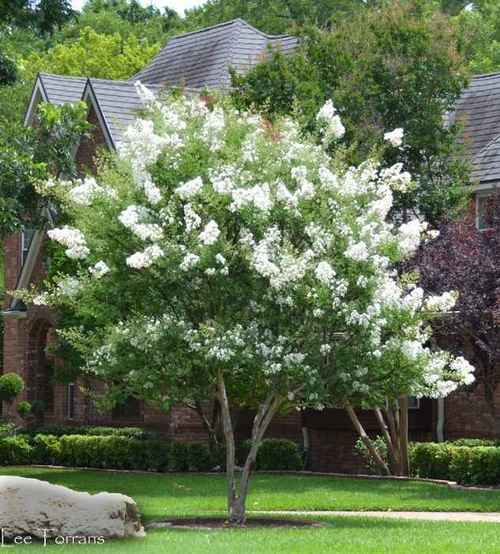
\includegraphics[width=\linewidth]{ZongJie/Appendix/MinCiJieShi/fig/XianZhi_CreepMyrtle}
     \caption{番石榴樹}
  \end{subfigure}
  \begin{subfigure}[b]{0.2\linewidth}
    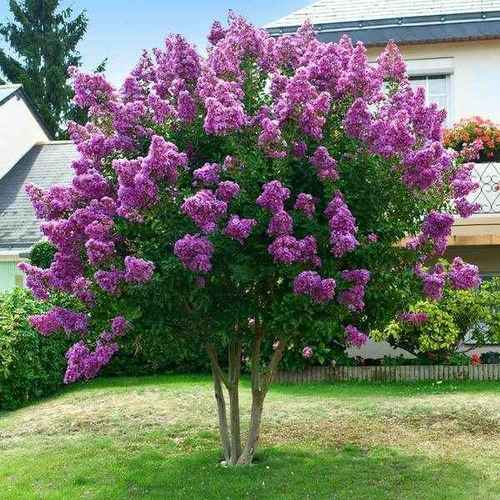
\includegraphics[width=\linewidth,height=3.9cm]{ZongJie/Appendix/MinCiJieShi/fig/XianZhi_CreepMyrtle2}
    \caption{番石榴樹}
  \end{subfigure}
  \begin{subfigure}[b]{0.2\linewidth}
    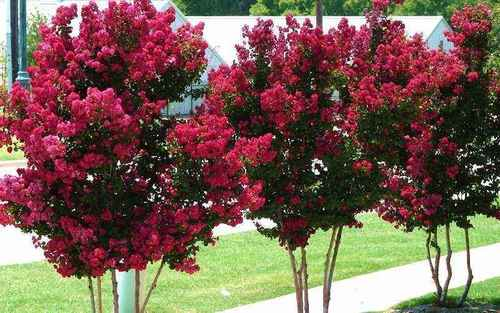
\includegraphics[width=\linewidth,height=3.85cm]{ZongJie/Appendix/MinCiJieShi/fig/XianZhi_CreepMyrtle3}
    \caption{番石榴樹}
  \end{subfigure}
\end{figure}







\subsection{愤怒 אַ֨ף  nostril, nose, face, anger（oftener divine）}
\subsubsection{其他书卷 אַ֨ף  nostril, nose, face, anger（oftener divine）}
\begin{itemize} 
\itemsep-.25em
\item 3 mostly anger, human Genesis 27:45; Genesis 49:6,7 + (45 t.); oftener divine Exodus 32:12; Deuteronomy 9:19; 2 Kings 24:20 + (177 t.); often subject חָרָה (וַיִּ֫חַר etc.) his anger was kindled Genesis 30:2; Genesis 39:19; Exodus 4:14; Exodus 22:23; Exodus 32:10,11 +; in various combinations, especially חֲרוֺן אַף fierceness of anger Exodus 32:12; Numbers 25:4; Numbers 32:14 +; compare חֳרִיאָֿף 1 Samuel 20:34; בַּעַלאַֿף Proverbs 22:24 one given to anger, etc.; אֶרֶךְ אַמַּיִם slow to anger Exodus 34:6; Numbers 14:18; Nehemiah 9:17 7t. of God; Proverbs 14:29; Proverbs 15:18; Proverbs 16:32; Proverbs 25:15 of man.
\item 出埃及記 22:24 並要發烈怒，用刀殺你們，使你們的妻子為寡婦，兒女為孤兒。
\item 民數記 16:46 摩西對亞倫說：「拿你的香爐，把壇上的火盛在其中，又加上香，快快帶到會眾那裡，為他們贖罪。因為有憤怒從耶和華那裡出來，瘟疫已經發作了。」
民數記 18:5 你們要看守聖所和壇，免得憤怒再臨到以色列人。
\item 歷代志下 36:16 他們卻戲笑神的使者，藐視他的言語，譏誚他的先知，以致耶和華的憤怒向他的百姓發作，無法可救。
\end{itemize}  

\subsubsection{詩篇}
\begin{itemize} 
\itemsep-.25em
\item 詩篇 88:7 你的憤怒重壓我身，你用一切的波浪困住我。（細拉）
\item 詩篇 89:46 耶和華啊，這要到幾時呢？你要將自己隱藏到永遠嗎？你的憤怒如火焚燒要到幾時呢？箴言 16:14 王的震怒如殺人的使者，但智慧人能止息王怒。
\item 詩篇 106:40 所以耶和華的怒氣向他的百姓發作，憎惡他的產業，
\item 詩篇 124:3 向我們發怒的時候，就把我們活活地吞了。
\end{itemize}  

\subsubsection{以賽亞書，耶利米哀歌，哈巴谷書}
\begin{itemize} 
\itemsep-.25em
\item 以賽亞書 13:13 我萬軍之耶和華在憤恨中發烈怒的日子，必使天震動，使地搖撼離其本位。
\item 以賽亞書 60:10 「外邦人必建築你的城牆，他們的王必服侍你。我曾發怒擊打你，現今卻施恩憐恤你。
\item 耶利米哀歌 3:1 我是因耶和華憤怒的杖遭遇困苦的人。
\item agitation, excitement, raging; — ׳ר absolute Habakkuk 3:2 +, construct Job 37:2; suffix רָנְזֶךָ֑ Isaiah 14:3; — raging Job 3:17; disquiet, turmoil Isaiah 14:3; Job 3:26; Job 14:1; raging, wrath Habakkuk 3:2; קֹלוֺ ׳ר Job 37:2 rumbling of his voice (i.e. thunder); of excitement of warhorse, בְּרַעַשׁ וְרֹגֶּז Job 39:24.
哈巴谷書 3:2 耶和華啊，我聽見你的名聲就懼怕。耶和華啊，求你在這些年間復興你的作為，在這些年間顯明出來，在發怒 的時候以憐憫為念。
\end{itemize}  

\subsubsection{羅馬書 2:5，9:22}
\begin{itemize} 
\itemsep-.25em
\item 羅馬書 2:5 你竟任著你剛硬不悔改的心，為自己積蓄憤怒，以致神震怒，顯他公義審判的日子來到。
\item 窯匠難道沒有權柄從一團泥裡拿一塊做成貴重的器皿，又拿一塊做成卑賤的器皿嗎？ 22倘若神要顯明他的憤怒，彰顯他的權能，就多多忍耐寬容那可怒、預備遭毀滅的器皿， 23又要將他豐盛的榮耀彰顯在那蒙憐憫、早預備得榮耀的器皿上
\end{itemize}  





\subsection{婦人}
\subsubsection{身披日頭，腳踏月亮，頭戴十二星冠冕的婦人}
天上現出大異象來：有一個婦人身披日頭，腳踏月亮，頭戴十二星的冠冕， 2 她懷了孕，在生產的艱難中疼痛呼叫。
\subsubsection{婦人的孩子被提到神寶座}
天上又現出異象來：有一條大紅龍，七頭十角，七頭上戴著七個冠冕， 4 牠的尾巴拖拉著天上星辰的三分之一，摔在地上。龍就站在那將要生產的婦人面前，等她生產之後，要吞吃她的孩子。 5 婦人生了一個男孩子，是將來要用鐵杖轄管 a萬國的；她的孩子被提到神寶座那裡去了。 6 婦人就逃到曠野，在那裡有神給她預備的地方，使她被養活一千二百六十天。

\subsubsection{撫養婦人一載二載半載}

13 龍見自己被摔在地上，就逼迫那生男孩子的婦人。 14 於是有大鷹的兩個翅膀賜給婦人，叫她能飛到曠野，到自己的地方躲避那蛇，她在那裡被養活一載，二載，半載。 15 蛇就在婦人身後，從口中吐出水來，像河一樣，要將婦人沖去。 16 地卻幫助婦人，開口吞了從龍口吐出來的水 b。 17 龍向婦人發怒，去與她其餘的兒女爭戰，這兒女就是那守神誡命、為耶穌作見證的。那時龍就站在海邊的沙上。

\subsection{大淫妇}
\subsubsection{大淫婦的刑罰 }
拿著七碗的七位天使中，有一位前來對我說：「你到這裡來，我將坐在眾水上的大淫婦所要受的刑罰指給你看。 2 地上的君王與她行淫，住在地上的人喝醉了她淫亂的酒。」 3 我被聖靈感動，天使帶我到曠野去。我就看見一個女人騎在朱紅色的獸上，那獸有七頭十角，遍體有褻瀆的名號。 4 那女人穿著紫色和朱紅色的衣服，用金子、寶石、珍珠為裝飾，手拿金杯，杯中盛滿了可憎之物，就是她淫亂的汙穢。 5 在她額上有名寫著說：「奧祕哉，大巴比倫，做世上的淫婦和一切可憎之物的母！」 6 我又看見那女人喝醉了聖徒的血和為耶穌作見證之人的血。我看見她，就大大地稀奇。
\subsubsection{大淫婦騎獸的奧祕}
天使又對我說：「你所看見那淫婦坐的眾水，就是多民、多人、多國、多方。 16 你所看見的那十角與獸必恨這淫婦，使她冷落赤身，又要吃她的肉，用火將她燒盡。 17 因為神使諸王同心合意，遵行他的旨意，把自己的國給那獸，直等到神的話都應驗了。 18 你所看見的那女人就是管轄地上眾王的大城。」


\subsubsection{巴比倫傾倒}

1 此後，我看見另有一位有大權柄的天使從天降下，地就因他的榮耀發光。 2 他大聲喊著說：「巴比倫大城傾倒了！傾倒了！成了鬼魔的住處和各樣汙穢之靈的巢穴 a，並各樣汙穢可憎之雀鳥的巢穴。 3 因為列國都被她邪淫大怒的酒傾倒了，地上的君王與她行淫，地上的客商因她奢華太過就發了財。」

\subsubsection{先有榮耀奢華後受悲哀痛苦}
我又聽見從天上有聲音說：「我的民哪，你們要從那城出來，免得與她一同有罪，受她所受的災殃。 5 因她的罪惡滔天，她的不義，神已經想起來了。 6 她怎樣待人，也要怎樣待她，按她所行的加倍地報應她，用她調酒的杯加倍地調給她喝。 7 她怎樣榮耀自己，怎樣奢華，也當叫她照樣痛苦悲哀；因她心裡說：『我坐了皇后的位，並不是寡婦，決不至於悲哀。』 8 所以在一天之內，她的災殃要一齊來到，就是死亡、悲哀、饑荒。她又要被火燒盡了，因為審判她的主神大有能力。 9 地上的君王，素來與她行淫、一同奢華的，看見燒她的煙，就必為她哭泣哀號。 10 因怕她的痛苦，就遠遠地站著說：『哀哉！哀哉！巴比倫大城，堅固的城啊，一時之間你的刑罰就來到了！』 11 地上的客商也都為她哭泣悲哀，因為沒有人再買他們的貨物了。 12 這貨物就是金、銀、寶石、珍珠、細麻布、紫色料、綢子、朱紅色料，各樣香木，各樣象牙的器皿，各樣極寶貴的木頭和銅、鐵、漢白玉的器皿， 13 並肉桂、豆蔻、香料、香膏、乳香、酒、油、細麵、麥子、牛、羊、車、馬和奴僕、人口。

\subsubsection{因大城受報應聖徒都歡喜}
「巴比倫哪，你所貪愛的果子離開了你，你一切的珍饈美味和華美的物件也從你中間毀滅，決不能再見了！ 15 販賣這些貨物，藉著她發了財的客商，因怕她的痛苦，就遠遠地站著哭泣悲哀， 16 說：『哀哉，哀哉，這大城啊！素常穿著細麻、紫色、朱紅色的衣服，又用金子、寶石和珍珠為裝飾， 17 一時之間，這麼大的富厚就歸於無有了！』凡船主和坐船往各處去的，並眾水手，連所有靠海為業的，都遠遠地站著， 18 看見燒她的煙就喊著說：『有何城能比這大城呢？』 19 他們又把塵土撒在頭上，哭泣悲哀，喊著說：『哀哉，哀哉，這大城啊！凡有船在海中的都因她的珍寶成了富足，她在一時之間就成了荒場！』 20 天哪，眾聖徒、眾使徒、眾先知啊！你們都要因她歡喜，因為神已經在她身上申了你們的冤。」

21 有一位大力的天使舉起一塊石頭，好像大磨石，扔在海裡說：「巴比倫大城也必這樣猛力地被扔下去，決不能再見了。 22 彈琴、作樂、吹笛、吹號的聲音在你中間決不能再聽見。各行手藝人在你中間決不能再遇見。推磨的聲音在你中間決不能再聽見。 23 燈光在你中間決不能再照耀。新郎和新婦的聲音在你中間決不能再聽見。你的客商原來是地上的尊貴人，萬國也被你的邪術迷惑了。 24 先知和聖徒並地上一切被殺之人的血，都在這城裡看見了。」

\subsubsection{神申討大淫婦流人血之罪}

1 此後，我聽見好像群眾在天上大聲說：「哈利路亞 a！救恩、榮耀、權能都屬乎我們的神！ 2 他的判斷是真實、公義的，因他判斷了那用淫行敗壞世界的大淫婦，並且向淫婦討流僕人血的罪，給他們申冤。」 3 又說：「哈利路亞！燒淫婦的煙往上冒，直到永永遠遠！」 4 那二十四位長老與四活物就俯伏敬拜坐寶座的神，說：「阿們！哈利路亞！」 5 有聲音從寶座出來，說：「神的眾僕人哪，凡敬畏他的，無論大小，都要讚美我們的神！」 6 我聽見好像群眾的聲音，眾水的聲音，大雷的聲音，說：「哈利路亞！因為主我們的神，全能者做王了。





  
\subsection{號trumpet， חֲצֹצְרֹת，שׁוֺפָר}
חֲצֹצְרָה noun feminine clarion (Late Hebrew חֲצוֺצֶרֶת, Aramaic חֲצוֺצַרְתָּצ) — mostly P and late; — absolute ׳ח Hosea 5:8; plural absolute חֲצֹצְרוֺת Numbers 10:8 22t.; חֲצֹצְרֹת Numbers 10:9,10; construct id. Numbers 31:6; 2Chronicles 13:12; חֲצוֺצְרֹת Numbers 10:2; clarion


as secular instr. Hosea 5:8 ("" שׁוֺפָר) 2 Kings 11:14 (twice in verse) = 2Chronicles 23:13 (twice in verse).

2 as sacred instr. 2 Kings 12:14, especially for use by priests (only P, Psalm 98 and Chronicles).

a. ׳תקע בח (of blowing a single long blast) Numbers 10:3,4,7,8, to gather congregation or ׳נשׂיא together, and, on festivals, over sacrifice, 'to be remembered before ׳י,' Numbers 10:10.

b. ׳תקע תרועה בח, or ׳הריע בח (of sounding alarm, — a series of quick blasts) for camps to move Numbers 10:5,6, also in battle, Numbers 10:9, 'to be remembered before ׳י;' so Numbers 31:6; 2Chronicles 13:12 (compare 2 Chronicles 13:14), both התרועה ׳ח.

c. especially in Chr's descriptions of ceremonies at festivals, to express rejoicing: 1 Chronicles 13:8; 1 Chronicles 15:28 ("" קוֺל שׁוֺפָר), 1 Chronicles 16:6,42; 2Chronicles 15:14 ("" שׁוֺפָר), 2 Chronicles 20:28; 29:26,27; Ezra 3:10; Nehemiah 12:35,41; Psalm 98:6 ("" קוֺל שׁוֺפָר); ׳הָרִים קוֺל בח2Chronicles 5:13; ׳מחצצרים בח 1 Chronicles 15:24; 2Chronicles 5:12,13; 13:14; in 2 Chronicles 29:28 this participle agrees with noun in sense, and is masculine; and the clarions (= players on the clarions) sounded. — The חֲצֹצְרָה, or (sacred) clarion, was a long, straight, slender metal tube, with flaring end, see BenzArchäol. 277; distinguished thus from the שׁוֺפָר which was originally a ram's horn, and probably always retained the horn-shape; the שׁוֺפָר is mentioned constantly in the earlier literature, and was used by watchmen, warriors, etc., as well as priests (see Benzib. 276 and שׁוֺפָר).

耶和華曉諭摩西說：「你要用銀子做兩枝號，都要錘出來的，用以招聚會眾，並叫眾營起行。吹這號的時候，全會眾要到你那裏，聚集在會幕門口。若單吹一枝，眾首領，就是以色列軍中的統領，要聚集到你那裏。吹出大聲的時候，東邊安的營都要起行。二次吹出大聲的時候，南邊安的營都要起行。他們將起行，必吹出大聲。但招聚會眾的時候，你們要吹號，卻不要吹出大聲。亞倫子孫作祭司的要吹這號；這要作你們世世代代永遠的定例。你們在自己的地，與欺壓你們的敵人打仗，就要用號吹出大聲，便在耶和華──你們的神面前得蒙紀念，也蒙拯救脫離仇敵。在你們快樂的日子和節期，並月朔，獻燔祭和平安祭，也要吹號，這都要在你們的神面前作為紀念，我是耶和華──你們的神。」（民數記十1～10）


另外，在特定的日子、節期和月朔，歡樂的場合中，他們也是吹奏銀號助興；就是每逢快樂的場合、各種節期、每月初一、每年的吹角節（民數記廿九1；利未記廿三24）、禧年的七月初十（利未記廿五9），各節期的宗教活動，也都要吹號。


吹號乃傳達最高神的命令，吹號的意義即表明傳揚神的聖言（參：馬可福音十六15；啟示錄十四6、7）。端視今日的基督徒在屬靈的曠野途中，有作戰，也有歡樂，有前進，也有等待，我們也是要藉著基督的號令，從四方招聚祂的百姓，並藉著基督的聖言，來帶領教會和幫助選民，祂是銀號的真體，是真理的發言者。

然而為宣告救贖之道，耶穌基督就像銀號一般，經由千錘百鍊，祂受盡了千辛萬苦，被神擊打苦待，才得以成全（希伯來書九12；以賽亞書五十三4～10），其目的就在宣揚救人之道，並對世人傳警告（參：馬太福音廿28；使徒行傳十三26）。


在歷代之中，選民所備的號並沒有局限幾枝；摩西之曠野時代，是選民最先設立吹號制度，他依耶和華神的吩咐，預備的銀號是兩枝。到了大衛的統一王國時期，就備有七枝號筒了（參：歷代志上十五24）。及至以色列國全盛時期，當時的所羅門王一口氣製造了120枝的號筒（歷代志下五12）。甚至末後基督再臨時，祂要差遣使者，用號筒的大聲，將祂的選民，從四方，從天這邊到天那邊，都招聚了來（參：馬太福音廿四31）。可見隨著時代的改變，不但使用號筒的數量跟著增加，而且也成了基督再臨的宣告。

因此，基督是那歷史以來，真正的呼召者，祂在古時以銀號呼召祂的百姓，今日更親自藉著教會，呼召末後的選民，祂的救贖的號聲是永不停頓，直到末日祂的再臨（啟示錄七9～17；馬太福音廿四30～31）。
今日的教會，必須嚴守歸回聖經的原則，傾聽基督的真理，分辨主的號聲，以恢復使徒時代的教會為標的，接受全備的教理，領受上頭澆灌的聖靈，確實傳揚神的聖言（馬可福音十六15；啟示錄十四6～7），

以西結書卅三1～9）。因此，要積極宣揚救贖之訊息，努力鼓吹，高舉基督的號角，盡祭司之職責（哥林多前書九16、17、19～22）





\subsection{患难，大患难2347: $\theta$$\lambda$$\widetilde{\iota}$$\psi$$\iota$$\varsigma$ θλῖψις}
\subsubsection{馬太福音 13:17-23 $\theta$$\lambda$$\acute{\iota}$$\psi$$\epsilon$$\omega$$\zeta$,24:3-14 $\theta$$\lambda$$\tilde{\iota}$$\psi$$\iota$$\nu$,24:20-31 $\theta$$\lambda$$\tilde{\iota}$$\psi$$\iota$$\zeta$ $\theta$$\lambda$$\tilde{\iota}$$\psi$$\iota$$\nu$}    
\begin{itemize} 
\itemsep-.25em
\item 17 「我實在告訴你們：從前有許多先知和義人要看你們所看的，卻沒有看見；要聽你們所聽的，卻沒有聽見。 18 所以，你們當聽這撒種的比喻： 19 凡聽見天國道理不明白的，那惡者就來，把所撒在他心裡的奪了去，這就是撒在路旁的了。 20 撒在石頭地上的，就是人聽了道，當下歡喜領受， 21 只因心裡沒有根，不過是暫時的，及至為道遭了\underline{患難$\theta$$\lambda$$\acute{\iota}$$\psi$$\epsilon$$\omega$$\zeta$}，或是受了逼迫，立刻就跌倒了。 22 撒在荊棘裡的，就是人聽了道，後來有世上的思慮、錢財的迷惑把道擠住了，不能結實。 23 撒在好地上的，就是人聽道明白了，後來結實，有一百倍的，有六十倍的，有三十倍的。」   
\item 耶穌在橄欖山上坐著，門徒暗暗地來，說：「請告訴我們，什麼時候有這些事？你降臨和世界的末了有什麼預兆呢？」 4 耶穌回答說：「你們要謹慎，免得有人迷惑你們。 5 因為將來有好些人冒我的名來，說：『我是基督』，並且要迷惑許多人。 6 你們也要聽見打仗和打仗的風聲，總不要驚慌，因為這些事是必須有的，只是末期還沒有到。 7 民要攻打民，國要攻打國，多處必有饑荒、地震， 8 這都是災難的起頭。 9 那時，人要把你們陷在\underline{患難$\theta$$\lambda$$\tilde{\iota}$$\psi$$\iota$$\nu$}裡，也要殺害你們；你們又要為我的名被萬民恨惡。「那時，必有許多人跌倒，也要彼此陷害、彼此恨惡， 11 且有好些假先知起來，迷惑多人。 12 只因不法的事增多，許多人的愛心才漸漸冷淡了。 13 唯有忍耐到底的，必然得救。 14 這天國的福音要傳遍天下，對萬民作見證，然後末期才來到。
\item 20 「你們應當祈求，叫你們逃走的時候，不遇見冬天或是安息日。 21 因為那時必有\underline{大災難$\theta$$\lambda$$\tilde{\iota}$$\psi$$\iota$$\zeta$}，從世界的起頭直到如今沒有這樣的災難，後來也必沒有。 22 若不減少那日子，凡有血氣的總沒有一個得救的；只是為選民，那日子必減少了。 23 那時，若有人對你們說『基督在這裡』，或說『基督在那裡』，你們不要信。 24 因為假基督、假先知將要起來，顯大神蹟、大奇事，倘若能行，連選民也就迷惑了。 25 看哪，我預先告訴你們了！ 26 若有人對你們說『看哪，基督在曠野裡』，你們不要出去；或說『看哪，基督在內屋中』，你們不要信。 27 閃電從東邊發出，直照到西邊，人子降臨也要這樣。 28 屍首在哪裡，鷹也必聚在那裡。「那些日子的\underline{災難$\theta$$\lambda$$\tilde{\iota}$$\psi$$\iota$$\nu$}一過去，『日頭就變黑了，月亮也不放光，眾星要從天上墜落，天勢都要震動。』 30 那時，人子的兆頭要顯在天上，地上的萬族都要哀哭。他們要看見人子有能力、有大榮耀駕著天上的雲降臨。 31 他要差遣使者，用號筒的大聲，將他的選民從四方，從天這邊到天那邊，都招聚了來。
\end{itemize}   
    
 \subsubsection{馬可福音 4:13-20 $\theta$$\lambda$$\acute{\iota}$$\psi$$\epsilon$$\omega$$\zeta$,13:14-27 $\theta$$\lambda$$\tilde{\iota}$$\psi$$\iota$$\zeta$, $\theta$$\lambda$$\tilde{\iota}$$\psi$$\iota$$\nu$} 
 \begin{itemize} 
\itemsep-.25em
\item {馬可福音 4:13-20}\\
13 又對他們說：「你們不明白這比喻嗎？這樣怎能明白一切的比喻呢？ 14 撒種之人所撒的就是道。 15 那撒在路旁的，就是人聽了道，撒旦立刻來，把撒在他心裡的道奪了去。 16 那撒在石頭地上的，就是人聽了道，立刻歡喜領受， 17 但他心裡沒有根，不過是暫時的，及至為道遭了\underline{患難$\theta$$\lambda$$\acute{\iota}$$\psi$$\epsilon$$\omega$$\zeta$}，或是受了逼迫，立刻就跌倒了。 18 還有那撒在荊棘裡的，就是人聽了道，19 後來有世上的思慮、錢財的迷惑和別樣的私慾進來，把道擠住了，就不能結實。 20 那撒在好地上的，就是人聽道又領受，並且結實，有三十倍的，有六十倍的，有一百倍的。」
\item{馬可福音 13:14-27}   \\
「你們看見『那行毀壞可憎的』站在不當站的地方——讀這經的人須要會意——那時，在猶太的，應當逃到山上； 15 在房上的，不要下來，也不要進去拿家裡的東西； 16 在田裡的，也不要回去取衣裳。 17 當那些日子，懷孕的和奶孩子的有禍了！ 18 你們應當祈求，叫這些事不在冬天臨到。 19 因為在那些日子必有\underline{災難$\theta$$\lambda$$\tilde{\iota}$$\psi$$\iota$$\zeta$}，自從神創造萬物直到如今並沒有這樣的災難，後來也必沒有。 20 若不是主減少那日子，凡有血氣的總沒有一個得救的；只是為主的選民，他將那日子減少了。 21 那時，若有人對你們說『看哪，基督在這裡』，或說『基督在那裡』，你們不要信。 22 因為假基督、假先知將要起來，顯神蹟奇事，倘若能行，就把選民迷惑了。 23 你們要謹慎！看哪，凡事我都預先告訴你們了！24 「在那些日子，那\underline{災難$\theta$$\lambda$$\tilde{\iota}$$\psi$$\iota$$\nu$}以後，『日頭要變黑了，月亮也不放光， 25 眾星要從天上墜落，天勢都要震動。』 26 那時，他們 b要看見人子有大能力、大榮耀駕雲降臨。 27 他要差遣天使，把他的選民從四方，從地極直到天邊，都招聚了來。  
\end{itemize}  

\subsubsection{約翰福音 16：19-33 $\theta$$\lambda$$\acute{\iota}$$\psi$$\epsilon$$\omega$$\varsigma$ $\theta$$\lambda$$\tilde{\iota}$$\psi$$\iota$$\nu$}
耶穌看出他們要問他，就說：「我說『等不多時，你們就不得見我；再等不多時，你們還要見我』，你們為這話彼此相問嗎？ 20 我實實在在地告訴你們：你們將要痛哭、哀號，世人倒要喜樂。你們將要憂愁，然而你們的憂愁要變為喜樂。 21 婦人生產的時候就憂愁，因為她的時候到了；既生了孩子，就不再記念那\underline{苦楚$\theta$$\lambda$$\acute{\iota}$$\psi$$\epsilon$$\omega$$\varsigma$}，因為歡喜世上生了一個人。 22 你們現在也是憂愁，但我要再見你們，你們的心就喜樂了，這喜樂也沒有人能奪去。23 「到那日，你們什麼也就不問我了。我實實在在地告訴你們：你們若向父求什麼，他必因我的名賜給你們。 24 向來你們沒有奉我的名求什麼，如今你們求，就必得著，叫你們的喜樂可以滿足。25 「這些事，我是用比喻對你們說的。時候將到，我不再用比喻對你們說，乃要將父明明地告訴你們。 26 到那日，你們要奉我的名祈求。我並不對你們說，我要為你們求父； 27 父自己愛你們，因為你們已經愛我，又信我是從父出來的。 28 我從父出來，到了世界；我又離開世界，往父那裡去。」 29 門徒說：「如今你是明說，並不用比喻了。 30 現在我們曉得你凡事都知道，也不用人問你，因此我們信你是從神出來的。」 31 耶穌說：「現在你們信嗎？ 32 看哪，時候將到，且是已經到了，你們要分散，各歸自己的地方去，留下我獨自一人；其實我不是獨自一人，因為有父與我同在。 33 我將這些事告訴你們，是要叫你們在我裡面有平安。在世上你們有\underline{苦難$\theta$$\lambda$$\tilde{\iota}$$\psi$$\iota$$\nu$}，但你們可以放心，我已經勝了世界。」


\subsubsection{使徒行傳 7:9-12 $\theta$$\lambda$$\tilde{\iota}$$\psi$$\iota$$\zeta$, 14:19-23 $\theta$$\lambda$$\acute{\iota}$$\psi$$\epsilon$$\omega$$\nu$, 20:17-24 $\theta$$\lambda$$\acute{\iota}$$\psi$$\epsilon$$\iota$$\zeta$} 
\begin{itemize} 
\itemsep-.25em
\item{使徒行傳 7:9-12}\\  9 先祖嫉妒約瑟，把他賣到埃及去。神卻與他同在， 10 救他脫離一切苦難，又使他在埃及王法老面前得恩典、有智慧。法老就派他做埃及國的宰相兼管全家。 11 後來埃及和迦南全地遭遇饑荒，大受\underline{艱難$\theta$$\lambda$$\tilde{\iota}$$\psi$$\iota$$\zeta$}，我們的祖宗就絕了糧。 12 雅各聽見在埃及有糧，就打發我們的祖宗初次往那裡去。
\item{使徒行傳 14:19-23} \\
 但有些猶太人從安提阿和以哥念來，挑唆眾人，就用石頭打保羅，以為他是死了，便拖到城外。 20 門徒正圍著他，他就起來，走進城去。第二天，同巴拿巴往特庇去。 21 對那城裡的人傳了福音，使好些人做門徒，就回路司得、以哥念、安提阿去， 22 堅固門徒的心，勸他們恆守所信的道，又說：「我們進入神的國，必須經歷許多\underline{艱難$\theta$$\lambda$$\acute{\iota}$$\psi$$\epsilon$$\omega$$\nu$}。」 23 二人在各教會中選立了長老，又禁食禱告，就把他們交託所信的主。
\item{使徒行傳 20:17-24} \\
保羅從米利都打發人往以弗所去，請教會的長老來。 18 他們來了，保羅就說：「你們知道自從我到亞細亞的日子以來，在你們中間始終為人如何， 19 服侍主凡事謙卑，眼中流淚，又因猶太人的謀害經歷試煉。 20 你們也知道，凡於你們有益的，我沒有一樣避諱不說的，或在眾人面前，或在各人家裡，我都教導你們。 21 又對猶太人和希臘人證明當向神悔改，信靠我主耶穌基督。 22 現在我往耶路撒冷去，心甚迫切，不知道在那裡要遇見什麼事。 23 但知道聖靈在各城裡向我指證，說有捆鎖與\underline{患難$\theta$$\lambda$$\acute{\iota}$$\psi$$\epsilon$$\iota$$\zeta$}等待我。 24 我卻不以性命為念，也不看為寶貴，只要行完我的路程，成就我從主耶穌所領受的職事，證明神恩惠的福音。 
 \end{itemize}
 
 
 \subsubsection{羅馬書 2：1-11 $\theta$$\lambda$$\widetilde{\iota}$$\psi$$\iota$$\varsigma$, 5:1-5 $\theta$$\lambda$$\acute{\iota}$$\psi$$\epsilon$$\sigma$$\iota$$\nu$ $\theta$$\lambda$$\tilde{\iota}$$\psi$$\iota$$\zeta$, 8:31-39 $\theta$$\lambda$$\tilde{\iota}$$\psi$$\iota$$\zeta$, 12:9-16 $\theta$$\lambda$$\acute{\iota}$$\psi$$\epsilon$$\iota$}
 \begin{itemize} 
\itemsep-.25em
\item{羅馬書 2：1-11}\\1 你這論斷人的，無論你是誰，也無可推諉。你在什麼事上論斷人，就在什麼事上定自己的罪，因你這論斷人的，自己所行卻和別人一樣。 2 我們知道這樣行的人，神必照真理審判他。 3 你這人哪，你論斷行這樣事的人，自己所行的卻和別人一樣，你以為能逃脫神的審判嗎？ 4 還是你藐視他豐富的恩慈、寬容、忍耐，不曉得他的恩慈是領你悔改呢？ 5 你竟任著你剛硬不悔改的心，為自己積蓄憤怒，以致神震怒，顯他公義審判的日子來到。 6 他必照各人的行為報應各人。 7 凡恆心行善，尋求榮耀、尊貴和不能朽壞之福的，就以永生報應他們； 8 唯有結黨、不順從真理反順從不義的，就以憤怒、惱恨報應他們。 9 將\underline{患難$\theta$$\lambda$$\widetilde{\iota}$$\psi$$\iota$$\varsigma$}、困苦加給一切作惡的人，先是猶太人，後是希臘人； 10 卻將榮耀、尊貴、平安加給一切行善的人，先是猶太人，後是希臘人。 11 因為神不偏待人。
\item{羅馬書 5:1-5} \\我們既因信稱義，就藉著我們的主耶穌基督得與神相和。 2 我們又藉著他，因信得進入現在所站的這恩典中，並且歡歡喜喜盼望神的榮耀。 3 不但如此，就是在\underline{患難$\theta$$\lambda$$\acute{\iota}$$\psi$$\epsilon$$\sigma$$\iota$$\nu$}中也是歡歡喜喜的。因為知道\underline{患難$\theta$$\lambda$$\tilde{\iota}$$\psi$$\iota$$\zeta$}生忍耐， 4 忍耐生老練，老練生盼望， 5 盼望不至於羞恥，因為所賜給我們的聖靈將神的愛澆灌在我們心裡。  
\item{羅馬書 8:31-39}   \\ 31 既是這樣，還有什麼說的呢？神若幫助我們，誰能敵擋我們呢？ 32 神既不愛惜自己的兒子，為我們眾人捨了，豈不也把萬物和他一同白白地賜給我們嗎？ 33 誰能控告神所揀選的人呢？有神稱他們為義了。 c 34 誰能定他們的罪呢？有基督耶穌已經死了，而且從死裡復活，現今在神的右邊，也替我們祈求。35 誰能使我們與基督的愛隔絕呢？難道是\underline{患難$\theta$$\lambda$$\tilde{\iota}$$\psi$$\iota$$\zeta$}嗎？是困苦嗎？是逼迫嗎？是飢餓嗎？是赤身露體嗎？是危險嗎？是刀劍嗎？ 36 如經上所記：「我們為你的緣故終日被殺，人看我們如將宰的羊。」 37 然而，靠著愛我們的主，在這一切的事上已經得勝有餘了。 38 因為我深信：無論是死，是生，是天使，是掌權的，是有能的，是現在的事，是將來的事， 39 是高處的，是低處的，是別的受造之物，都不能叫我們與神的愛隔絕；這愛是在我們的主基督耶穌裡的。 
 \item{羅馬書 12:9-16} \\ 愛人不可虛假；惡要厭惡，善要親近。 10 愛弟兄，要彼此親熱；恭敬人，要彼此推讓。 11 殷勤不可懶惰；要心裡火熱，常常服侍主。 12 在指望中要喜樂，在\underline{患難$\theta$$\lambda$$\acute{\iota}$$\psi$$\epsilon$$\iota$}中要忍耐，禱告要恆切。 13 聖徒缺乏要幫補，客要一味地款待。 14 逼迫你們的，要給他們祝福；只要祝福，不可咒詛。 15 與喜樂的人要同樂，與哀哭的人要同哭。 16 要彼此同心；不要志氣高大，倒要俯就卑微的人；不要自以為聰明。 
\end{itemize}
 
 
\subsubsection{哥林多前書 7：26-31 $\theta$$\lambda$$\tilde{\iota}$$\psi$$\iota$$\nu$} 
26 因現今的艱難，據我看來，人不如守素安常才好。 27 你有妻子纏著呢，就不要求脫離；你沒有妻子纏著呢，就不要求妻子。 28 你若娶妻，並不是犯罪；處女若出嫁，也不是犯罪。然而這等人肉身必受\underline{苦難$\theta$$\lambda$$\tilde{\iota}$$\psi$$\iota$$\nu$}，我卻願意你們免這苦難。 29 弟兄們，我對你們說，時候減少了。從此以後，那有妻子的，要像沒有妻子； 30 哀哭的，要像不哀哭；快樂的，要像不快樂；置買的，要像無有所得； 31 用世物的，要像不用世物；因為這世界的樣子將要過去了。
 
 
\subsubsection{林後 1:3-11 $\theta$$\lambda$$\acute{\iota}$$\psi$$\epsilon$$\iota$ $\theta$$\lambda$$\acute{\iota}$$\psi$$\epsilon$$\omega$$\zeta$,  2:1-4/4:16-18 $\theta$$\lambda$$\acute{\iota}$$\psi$$\epsilon$$\omega$$\zeta$, 6:1-10 $\theta$$\lambda$$\acute{\iota}$$\psi$$\epsilon$$\sigma$$\iota$$\nu$,  7:2-4 $\theta$$\lambda$$\acute{\iota}$$\psi$$\epsilon$$\iota$, 8:1-8 $\theta$$\lambda$$\acute{\iota}$$\psi$$\epsilon$$\omega$$\zeta$}
\begin{itemize} 
\itemsep-.25em
\item{哥林多後書 1：3-11}\\ 願頌讚歸於我們的主耶穌基督的父神，就是發慈悲的父，賜各樣安慰的神！ 4 我們在一切\underline{患難$\theta$$\lambda$$\acute{\iota}$$\psi$$\epsilon$$\iota$}中，他就安慰我們，叫我們能用神所賜的安慰去安慰那遭各樣患難的人。 5 我們既多受基督的苦楚，就靠基督多得安慰。 6 我們受患難呢，是為叫你們得安慰、得拯救；我們得安慰呢，也是為叫你們得安慰。這安慰能叫你們忍受我們所受的那樣苦楚。 7 我們為你們所存的盼望是確定的，因為知道你們既是同受苦楚，也必同得安慰。 8 弟兄們，我們不要你們不曉得，我們從前在亞細亞遭遇\underline{苦難$\theta$$\lambda$$\acute{\iota}$$\psi$$\epsilon$$\omega$$\zeta$}，被壓太重，力不能勝，甚至連活命的指望都絕了， 9 自己心裡也斷定是必死的，叫我們不靠自己，只靠叫死人復活的神。 10 他曾救我們脫離那極大的死亡，現在仍要救我們，並且我們指望他將來還要救我們。 11 你們以祈禱幫助我們，好叫許多人為我們謝恩，就是為我們因許多人所得的恩。
\item{哥林多後書 2：1-4} \\ 1 我自己定了主意，再到你們那裡去，必須大家沒有憂愁。 2 倘若我叫你們憂愁，除了我叫那憂愁的人以外，誰能叫我快樂呢？ 3 我曾把這事寫給你們，恐怕我到的時候，應該叫我快樂的那些人反倒叫我憂愁。我也深信，你們眾人都以我的快樂為自己的快樂。 4 我先前心裡\underline{難過$\theta$$\lambda$$\acute{\iota}$$\psi$$\epsilon$$\omega$$\zeta$}痛苦，多多地流淚寫信給你們，不是叫你們憂愁，乃是叫你們知道我格外地疼愛你們。
\item{哥林多後書 4：16-18} \\ 16 所以我們不喪膽，外體雖然毀壞，內心卻一天新似一天。 17 我們這至暫至輕的\underline{苦楚$\theta$$\lambda$$\acute{\iota}$$\psi$$\epsilon$$\omega$$\zeta$}，要為我們成就極重無比、永遠的榮耀。 18 原來我們不是顧念所見的，乃是顧念所不見的，因為所見的是暫時的，所不見的是永遠的。     
\item{哥林多後書 6：1-10} \\1 我們與神同工的，也勸你們不可徒受他的恩典。 2 因為他說：「在悅納的時候，我應允了你；在拯救的日子，我搭救了你。」看哪，現在正是悅納的時候！現在正是拯救的日子！ 3 我們凡事都不叫人有妨礙，免得這職分被人毀謗； 4 反倒在各樣的事上表明自己是神的用人，就如在許多的忍耐，\underline{患難$\theta$$\lambda$$\acute{\iota}$$\psi$$\epsilon$$\sigma$$\iota$$\nu$}，窮乏，困苦， 5 鞭打，監禁，擾亂，勤勞，警醒，不食， 6 廉潔，知識，恆忍，恩慈，聖靈的感化，無偽的愛心， 7 真實的道理，神的大能；仁義的兵器在左在右， 8 榮耀羞辱，惡名美名；似乎是誘惑人的，卻是誠實的； 9 似乎不為人所知，卻是人所共知的；似乎要死，卻是活著的；似乎受責罰，卻是不致喪命的； 10 似乎憂愁，卻是常常快樂的；似乎貧窮，卻是叫許多人富足的；似乎一無所有，卻是樣樣都有的。    
 \item{哥林多後書 7：2-4}   \\ 2 你們要心地寬大收納我們。我們未曾虧負誰，未曾敗壞誰，未曾占誰的便宜。 3 我說這話不是要定你們的罪，我已經說過，你們常在我們心裡，情願與你們同生同死。 4 我大大地放膽，向你們說話；我因你們多多誇口，滿得安慰，我們在一切\underline{患難$\theta$$\lambda$$\acute{\iota}$$\psi$$\epsilon$$\iota$}中分外地快樂。 
 \item{哥林多後書 8：1-8}   \\弟兄們，我把神賜給馬其頓眾教會的恩告訴你們， 2 就是他們在患難中受\underline{大試煉$\theta$$\lambda$$\acute{\iota}$$\psi$$\epsilon$$\omega$$\zeta$}的時候，仍有滿足的快樂，在極窮之間還格外顯出他們樂捐的厚恩。 3 我可以證明他們是按著力量，而且也過了力量，自己甘心樂意地捐助， 4 再三地求我們，准他們在這供給聖徒的恩情上有份。 5 並且他們所做的，不但照我們所想望的，更照神的旨意，先把自己獻給主，又歸附了我們。 6 因此我勸提多，既然在你們中間開辦這慈惠的事，就當辦成了。 7 你們既然在信心、口才、知識、熱心和待我們的愛心上，都格外顯出滿足來，就當在這慈惠的事上也格外顯出滿足來。 8 我說這話，不是吩咐你們，乃是藉著別人的熱心試驗你們愛心的實在。    
\end{itemize}
 
 
 
 \subsubsection{以弗所書 3:2-13 $\theta$$\lambda$$\acute{\iota}$$\psi$$\epsilon$$\sigma$$\acute{\iota}$$\nu$} 
 2 諒必你們曾聽見神賜恩給我，將關切你們的職分託付我， 3 用啟示使我知道福音的奧祕，正如我以前略略寫過的。 4 你們念了，就能曉得我深知基督的奧祕。 5 這奧祕在以前的世代沒有叫人知道，像如今藉著聖靈啟示他的聖使徒和先知一樣。 6 這奧祕就是外邦人在基督耶穌裡，藉著福音，得以同為後嗣，同為一體，同蒙應許。 7 我做了這福音的執事，是照神的恩賜，這恩賜是照他運行的大能賜給我的。 8 我本來比眾聖徒中最小的還小，然而他還賜我這恩典，叫我把基督那測不透的豐富傳給外邦人， 9 又使眾人都明白，這歷代以來隱藏在創造萬物之神裡的奧祕是如何安排的， 10 為要藉著教會，使天上執政的、掌權的現在得知神百般的智慧。 11 這是照神從萬世以前在我們主基督耶穌裡所定的旨意。 12 我們因信耶穌，就在他裡面放膽無懼，篤信不疑地來到神面前。 13 所以，我求你們不要因我為你們所受的\underline{患難$\theta$$\lambda$$\acute{\iota}$$\psi$$\epsilon$$\sigma$$\acute{\iota}$$\nu$}喪膽，這原是你們的榮耀。
 
 
 \subsubsection{腓立比書 1：12-17 $\theta$$\lambda$$\widetilde{\iota}$$\psi$$\iota$$\nu$, 4：10-14 $\theta$$\lambda$$\acute{\iota}$$\psi$$\epsilon$$\iota$}
 \begin{itemize} 
\itemsep-.25em
\item{腓立比書 1：12-17}\\ 12 弟兄們，我願意你們知道，我所遭遇的事更是叫福音興旺， 13 以致我受的捆鎖在御營全軍和其餘的人中，已經顯明是為基督的緣故； 14 並且那在主裡的弟兄，多半因我受的捆鎖就篤信不疑，越發放膽傳神的道，無所懼怕。 15 有的傳基督是出於嫉妒紛爭，也有的是出於好意。 16 這一等是出於愛心，知道我是為辯明福音設立的； 17 那一等傳基督是出於結黨，並不誠實，意思要加增我捆鎖的\underline{苦楚$\theta$$\lambda$$\widetilde{\iota}$$\psi$$\iota$$\nu$}。
 \begin{cjhebrew}
hr.s  .S.hl  r.s  צַר, לַחַץ,צָרָה 
 \end{cjhebrew}
 \item{腓立比書 4：10-14}\\ 10 我靠主大大地喜樂，因為你們思念我的心如今又發生；你們向來就思念我，只是沒得機會。 11 我並不是因缺乏說這話，我無論在什麼景況都可以知足，這是我已經學會了。 12 我知道怎樣處卑賤，也知道怎樣處豐富，或飽足或飢餓，或有餘或缺乏，隨事隨在，我都得了祕訣。 13 我靠著那加給我力量的，凡事都能做。 14 然而，你們和我同受\underline{患難$\theta$$\lambda$$\acute{\iota}$$\psi$$\epsilon$$\iota$}原是美事。
 \end{itemize}
 
 
 \subsubsection{歌羅西書 1：23-27 $\theta$$\lambda$$\acute{\iota}$$\psi$$\epsilon$$\omega$$\nu$}
 23 只要你們在所信的道上恆心，根基穩固，堅定不移，不致被引動失去福音的盼望。這福音就是你們所聽過的，也是傳於普天下萬人聽的。我保羅也做了這福音的執事。24 現在我為你們受苦，倒覺歡樂，並且為基督的身體，就是為教會，要在我肉身上補滿基督\underline{患難$\theta$$\lambda$$\acute{\iota}$$\psi$$\epsilon$$\omega$$\nu$}的缺欠。 25 我照神為你們所賜我的職分做了教會的執事，要把神的道理傳得全備。 26 這道理就是歷世歷代所隱藏的奧祕，但如今向他的聖徒顯明了。 27 神願意叫他們知道，這奧祕在外邦人中有何等豐盛的榮耀，就是基督在你們心裡成了有榮耀的盼望。
 
 \subsubsection{帖前 1:2-8 $\theta$$\lambda$$\acute{\iota}$$\psi$$\epsilon$$\iota$, 3:1-10 $\theta$$\lambda$$\acute{\iota}$$\psi$$\epsilon$$\sigma$$\iota$$\nu$ $\theta$$\lambda$$\acute{\iota}$$\beta$$\epsilon$$\sigma$$\theta$$\alpha$$\iota$$\tau$$o$ $\theta$$\lambda$$\acute{\iota}$$\psi$$\epsilon$$\iota$, 帖後 1:3-10 $\theta$$\lambda$$\acute{\iota}$$\psi$$\epsilon$$\sigma$$\iota$$\nu$ $\theta$$\lambda$$\tilde{\iota}$$\psi$$\iota$$\nu$} 
 \begin{itemize} 
\itemsep-.25em
\item{帖撒羅尼迦前書}\\ 2 我們為你們眾人常常感謝神，禱告的時候提到你們， 3 在神我們的父面前不住地記念你們因信心所做的工夫，因愛心所受的勞苦，因盼望我們主耶穌基督所存的忍耐。 4 被神所愛的弟兄啊，我知道你們是蒙揀選的， 5 因為我們的福音傳到你們那裡，不獨在乎言語，也在乎權能和聖靈並充足的信心。正如你們知道，我們在你們那裡，為你們的緣故是怎樣為人。 6 並且你們在\underline{大難 plural $\theta$$\lambda$$\acute{\iota}$$\psi$$\epsilon$$\iota$}之中蒙了聖靈所賜的喜樂，領受真道，就效法我們，也效法了主， 7 甚至你們做了馬其頓和亞該亞所有信主之人的榜樣。 8 因為主的道從你們那裡已經傳揚出來，你們向神的信心不但在馬其頓和亞該亞，就是在各處也都傳開了，所以不用我們說什麼話。
 \item{帖撒羅尼迦前書 3:1-10}\\
 1 我們既不能再忍，就願意獨自等在雅典， 2 打發我們的兄弟——在基督福音上做神執事的提摩太前去，堅固你們，並在你們所信的道上勸慰你們， 3 免得有人被諸般\underline{患難$\theta$$\lambda$$\acute{\iota}$$\psi$$\epsilon$$\sigma$$\iota$$\nu$}搖動。因為你們自己知道，我們受患難原是命定的。 4 我們在你們那裡的時候，預先告訴你們我們\underline{必受患難$\theta$$\lambda$$\acute{\iota}$$\beta$$\epsilon$$\sigma$$\theta$$\alpha$$\iota$$\tau$$o$ (to suffer tribulation)}，以後果然應驗了，你們也知道。 5 為此，我既不能再忍，就打發人去，要曉得你們的信心如何，恐怕那誘惑人的到底誘惑了你們，叫我們的勞苦歸於徒然。 6 但提摩太剛才從你們那裡回來，將你們信心和愛心的好消息報給我們，又說你們常常記念我們，切切地想見我們，如同我們想見你們一樣。 7 所以弟兄們，我們在一切困苦\underline{患難$\theta$$\lambda$$\acute{\iota}$$\psi$$\epsilon$$\iota$}之中，因著你們的信心就得了安慰。 8 你們若靠主站立得穩，我們就活了。 9 我們在神面前，因著你們甚是喜樂，為這一切喜樂，可用何等的感謝為你們報答神呢！ 10 我們晝夜切切地祈求，要見你們的面，補滿你們信心的不足。
 \item{帖後 1:3-10}\\ 3 弟兄們，我們該為你們常常感謝神，這本是合宜的，因你們的信心格外增長，並且你們眾人彼此相愛的心也都充足。 4 甚至我們在神的各教會裡為你們誇口，都因你們在所受的一切逼迫\underline{患難$\theta$$\lambda$$\acute{\iota}$$\psi$$\epsilon$$\sigma$$\iota$$\nu$}中，仍舊存忍耐和信心。 5 這正是神公義判斷的明證，叫你們可算配得神的國，你們就是為這國受苦。 6 神既是公義的，就必將患難報應那加\underline{患難$\theta$$\lambda$$\tilde{\iota}$$\psi$$\iota$$\nu$}給你們的人， 7 也必使你們這受患難的人與我們同得平安。那時，主耶穌同他有能力的天使從天上在火焰中顯現， 8 要報應那不認識神和那不聽從我主耶穌福音的人。 9 他們要受刑罰，就是永遠沉淪，離開主的面和他權能的榮光。 10 這正是主降臨，要在他聖徒的身上得榮耀，又在一切信的人身上顯為稀奇的那日子。我們對你們作的見證，你們也信了。
\end{itemize}
       

\subsubsection{希伯來書 10:32-39 $\theta$$\lambda$$\acute{\iota}$$\psi$$\epsilon$$\sigma$$\iota$$\nu$} 
 32 你們要追念往日蒙了光照以後，所忍受大爭戰的各樣苦難。 33 一面被毀謗，遭\underline{患難$\theta$$\lambda$$\acute{\iota}$$\psi$$\epsilon$$\sigma$$\iota$$\nu$}，成了戲景叫眾人觀看；一面陪伴那些受這樣苦難的人。 34 因為你們體恤了那些被捆鎖的人，並且你們的家業被人搶去，也甘心忍受，知道自己有更美、長存的家業。 35 所以，你們不可丟棄勇敢的心，存這樣的心必得大賞賜。 36 你們必須忍耐，使你們行完了神的旨意，就可以得著所應許的。 37 「因為還有一點點時候，那要來的就來，並不遲延。 38 只是義人 b必因信得生；他若退後，我心裡就不喜歡他。」 39 我們卻不是退後入沉淪的那等人，乃是有信心以致靈魂得救的人。
  
 \subsubsection{雅各書 1:26-27 $\theta$$\lambda$$\acute{\iota}$$\psi$$\epsilon$$\iota$}   
 26 若有人自以為虔誠，卻不勒住他的舌頭，反欺哄自己的心，這人的虔誠是虛的。 27 在神我們的父面前，那清潔沒有玷汙的虔誠就是看顧在\underline{患難$\theta$$\lambda$$\acute{\iota}$$\psi$$\epsilon$$\iota$}中的孤兒寡婦，並且保守自己不沾染世俗。   
 
 \subsubsection{啟示錄 1:9-11 $\theta$$\lambda$$\acute{\iota}$$\psi$$\epsilon$$\iota$, 2:8-11 $\theta$$\lambda$$\tilde{\iota}$$\psi$$\iota$$\nu$, 2:18-23 $\theta$$\lambda$$\tilde{\iota}$$\psi$$\iota$$\nu$, 7:13-17 $\theta$$\lambda$$\acute{\iota}$$\psi$$\epsilon$$\omega$$\zeta$} 
  \begin{itemize} 
\itemsep-.25em
\item{啟示錄 1:9-11}\\
 我約翰，就是你們的弟兄，和你們在耶穌的\underline{患難$\theta$$\lambda$$\acute{\iota}$$\psi$$\epsilon$$\iota$}、國度、忍耐裡一同有份，為神的道並為給耶穌作的見證，曾在那名叫拔摩的海島上。 10 當主日，我被聖靈感動，聽見在我後面有大聲音如吹號說： 11 「你所看見的當寫在書上，達於以弗所、士每拿、別迦摩、推雅推喇、撒狄、非拉鐵非、老底嘉那七個教會。」   
    
\item{啟示錄 2:8-11} \\ 
你要寫信給士每拿教會的使者說：『那首先的、末後的、死過又活的說： 9 我知道你的患難、你的貧窮，你卻是富足的；也知道那自稱是猶太人所說的毀謗話，其實他們不是猶太人，乃是撒旦一會的人。10 『你將要受的苦你不用怕。魔鬼要把你們中間幾個人下在監裡，叫你們被試煉，你們必受\underline{患難$\theta$$\lambda$$\tilde{\iota}$$\psi$$\iota$$\nu$}十日。你務要至死忠心，我就賜給你那生命的冠冕。 11 聖靈向眾教會所說的話，凡有耳的，就應當聽！得勝的，必不受第二次死的害。』

\item{啟示錄 2:18-23}   \\       
  18 「你要寫信給推雅推喇教會的使者說：『那眼目如火焰、腳像光明銅的神之子說： 19 我知道你的行為、愛心、信心、勤勞、忍耐，又知道你末後所行的善事比起初所行的更多。 20 然而，有一件事我要責備你，就是你容讓那自稱是先知的婦人耶洗別教導我的僕人，引誘他們行姦淫，吃祭偶像之物。 21 我曾給她悔改的機會，她卻不肯悔改她的淫行。 22 看哪，我要叫她病臥在床；那些與她行淫的人，若不悔改所行的，我也要叫他們同受\underline{大患難$\theta$$\lambda$$\tilde{\iota}$$\psi$$\iota$$\nu$}。 23 我又要殺死她的黨類 a，叫眾教會知道我是那察看人肺腑心腸的，並要照你們的行為報應你們各人。   
 \item{啟示錄 7:13-17} \\    
  13 長老中有一位問我說：「這些穿白衣的是誰？是從哪裡來的？」 14 我對他說：「我主，你知道。」他向我說：「這些人是從\underline{大患難$\theta$$\lambda$$\acute{\iota}$$\psi$$\epsilon$$\omega$$\zeta$}中出來的，曾用羔羊的血把衣裳洗白淨了。 15 所以，他們在神寶座前，晝夜在他殿中侍奉他；坐寶座的要用帳幕覆庇他們。 16 他們不再飢、不再渴，日頭和炎熱也必不傷害他們， 17 因為寶座中的羔羊必牧養他們，領他們到生命水的泉源；神也必擦去他們一切的眼淚。」   
\end{itemize}










